
\newpage
\appendix

\section*{Appendices}
\startcontents[appendix]

All videos are available at \website

\section*{Appendix Outline}
\printcontents[appendix]{}{1}{\setcounter{tocdepth}{2}}

\section{Environment Creation}


% \begin{figure}
%     \centering
%     \includegraphics[width=0.5\linewidth]{corl_2026_template_submission/figures/example/PLD_operation.pdf}
%     \caption{GPU insertion placeholder}
%     \label{fig:gpu_insert_dr}
% \end{figure}














% token stats
% multi modality
% harness

% video
% push t - heuristic [whole process]
% pin insertion - online rl  [whole process]
% gpu 
% zip tie cut: vla + gofe
% zip tie insertion: offline RL


%release:
%drone shot: 



\subsection{Autonomous Reset}
We show that, given a task specification, coding agents can synthesize long-horizon reset functions by composing perception and planning APIs, including SAM3 for open-vocabulary object detection (illustrated in \Cref{fig:sam3_api}), BundleSDF for continuous 6-DOF pose tracking, and cuRobo for GPU-accelerated collision-free trajectory optimization. During execution, these reset functions consume real-time RGBD streams and proprioceptive state, which together support robust object localization, grasp pose generation, and motion planning. Coding agents can also command and read gripper torque signals, which serve as a surrogate for tactile feedback; we find that these signals are crucial for slip detection and controlling the force of the grip in precision-critical manipulation tasks.

\captionof{codesnippet}{\textbf{Tool API: SAM3 Multi-Object Segmentation.} Detects all instances of a queried object from a chosen camera view, returning per-instance masks, confidence scores, and back-projected 3D centroids.}
\label{fig:sam3_api}
\begin{appendixcode}{python}
class SegmentAllObjectsTool(Tool):
    """Detect all instances of an object using SAM3 multi-detection."""
    parameters = [
        ToolParameter("query",                "str"),
        ToolParameter("camera",               "str",   default="top"),
        ToolParameter("score_thresh",         "float", default=0.1),
        ToolParameter("image_bbox",           "list",  default=None),
        ToolParameter("image_exclude_bboxes", "list",  default=None),
        ToolParameter("filters",              "list",  default=None),
        ToolParameter("rank_by",              "dict",  default=None),
    ]
    # query:
    #     Natural-language description of the object to segment.
    # camera:
    #     Camera view to capture from. One of {top, left, right}.
    # score_thresh:
    #     Minimum SAM3 confidence score. Detections below threshold are dropped.
    # image_bbox:
    #     [x_min, y_min, x_max, y_max] pixel crop. Zeros all pixels outside the
    #     box before sending to SAM3 to suppress background noise. Returned masks
    #     remain in full-image coordinates so centroid_world_xyz back-projects correctly.
    # image_exclude_bboxes:
    #     List of [x_min, y_min, x_max, y_max] boxes to zero out before sending to
    #     SAM3. Inverse of image_bbox — used to blank known distractors (e.g. gripper
    #     jaws). Combinable with image_bbox: image_bbox is applied first, then
    #     exclusions zero out within the kept region.
    # filters:
    #     List of {metric, op, value} dicts AND-ed together to prune detections.
    #     metric in {confidence, area, AR, C, P}; op in {>=, <=}.
    #     AR: aspect ratio; C: compactness 4*pi*area/P^2; P: perimeter in pixels.
    #     Detections with None or non-finite metric values are dropped.
    # rank_by:
    #     {metric, direction} dict controlling sort order of returned detections.
    #     metric in {confidence, area, AR, C, P}; direction in {max, min}.
    #     Default: {confidence, max}.

    def execute(self, **kwargs) -> ToolResult:
        rgb         = self._fetch_camera_image(kwargs["camera"])
        rgb_for_sam = self._preprocess(rgb, kwargs["image_bbox"],
                                       kwargs["image_exclude_bboxes"])
        detections  = requests.post(f"{self._sam3_url}/segment_all",
                          json={"text":           kwargs["query"],
                                "image_b64":      to_b64(rgb_for_sam),
                                "score_threshold":kwargs["score_thresh"]}).json()
        depth, intr, T_cam_world = _fetch_camera_params(self._cam, kwargs["camera"])
        results = [
            SegmentationResult(
                mask               = np.load(io.BytesIO(base64.b64decode(d["mask_b64"]))),
                score              = d["score"],
                bbox_xywh          = d["bbox_xywh"],
                mask_area          = d["mask_area"],
                perimeter_px       = _shape_stats(mask)["perimeter_px"],
                compactness        = _shape_stats(mask)["compactness"],
                centroid_uv        = _shape_stats(mask)["centroid_uv"],
                centroid_world_xyz = _project_centroid(mask, depth, intr, T_cam_world),
                depth_m            = depth[v, u],
            ) for d in detections
        ]
        return ToolResult(success=True,
                          data=_rank_results(_apply_filters(results,
                                             kwargs["filters"]), kwargs["rank_by"]))
\end{appendixcode}

\vspace{0.5cm}
From these API tools, coding agents can synthesize perception skills such as semantic segmentation and 3D bounding box generation, as well as manipulation skills including pick-and-place, object reorientation, localization, and bimanual handover. Composing these skills with failure detection and retry mechanisms yields long-horizon reset functions that are robust to real-world perturbations. \Cref{fig:gpu_reset_policy} illustrates a concrete example for the GPU insertion task, where the agent sequences SAM3-based object localization, RANSAC~\cite{ransac} and OBB~\cite{obb}-based 3D bounding box estimation, torque-verified grasping, and cuRobo collision-free handover into a complete reset pipeline. Visualizations of the intermediate segmentation and bounding box outputs are provided in \Cref{fig:visual_tools_gpu_insertion}.




\captionof{codesnippet}{\textbf{Reset Policy: GPU Insertion Recovery.} Localizes the motherboard and target slot with SAM3, grasps and extracts the GPU with a torque-verified grip, then carries it to a parking pose via a cuRobo collision-free handover.}
\label{fig:gpu_reset_policy}
\begin{appendixcode}{python}
def reset_gpu_insertion():
    go_home()

    # --- SAM3: localize motherboard and target PCIe slot ---
    scene = sam3_localize_motherboard(camera="top")
    hover_pos, scene = acquire_slot_hover(scene)

    # --- grasp GPU and extract from slot ---
    descend_guided(scene)
    close_gripper(torque_limit=LEFT_CLOSE_TORQUE_LIMIT)
    verify_grasp_or_raise()                              # gripper torque check
    lift_and_pull(scene)

    # --- handover: carry GPU to parking pose on table ---
    freespace_move(left_target_pos=TABLE_APPROACH_POS,
                   left_target_rpy=TABLE_PLACE_RPY,
                   backend="curobo")
    release_glide(TABLE_PLACE_POS, TABLE_PLACE_RPY)     # synchronized open
    cartesian_retract_after_release()
    go_home()
\end{appendixcode}


\begin{figure}[H]
    \centering
    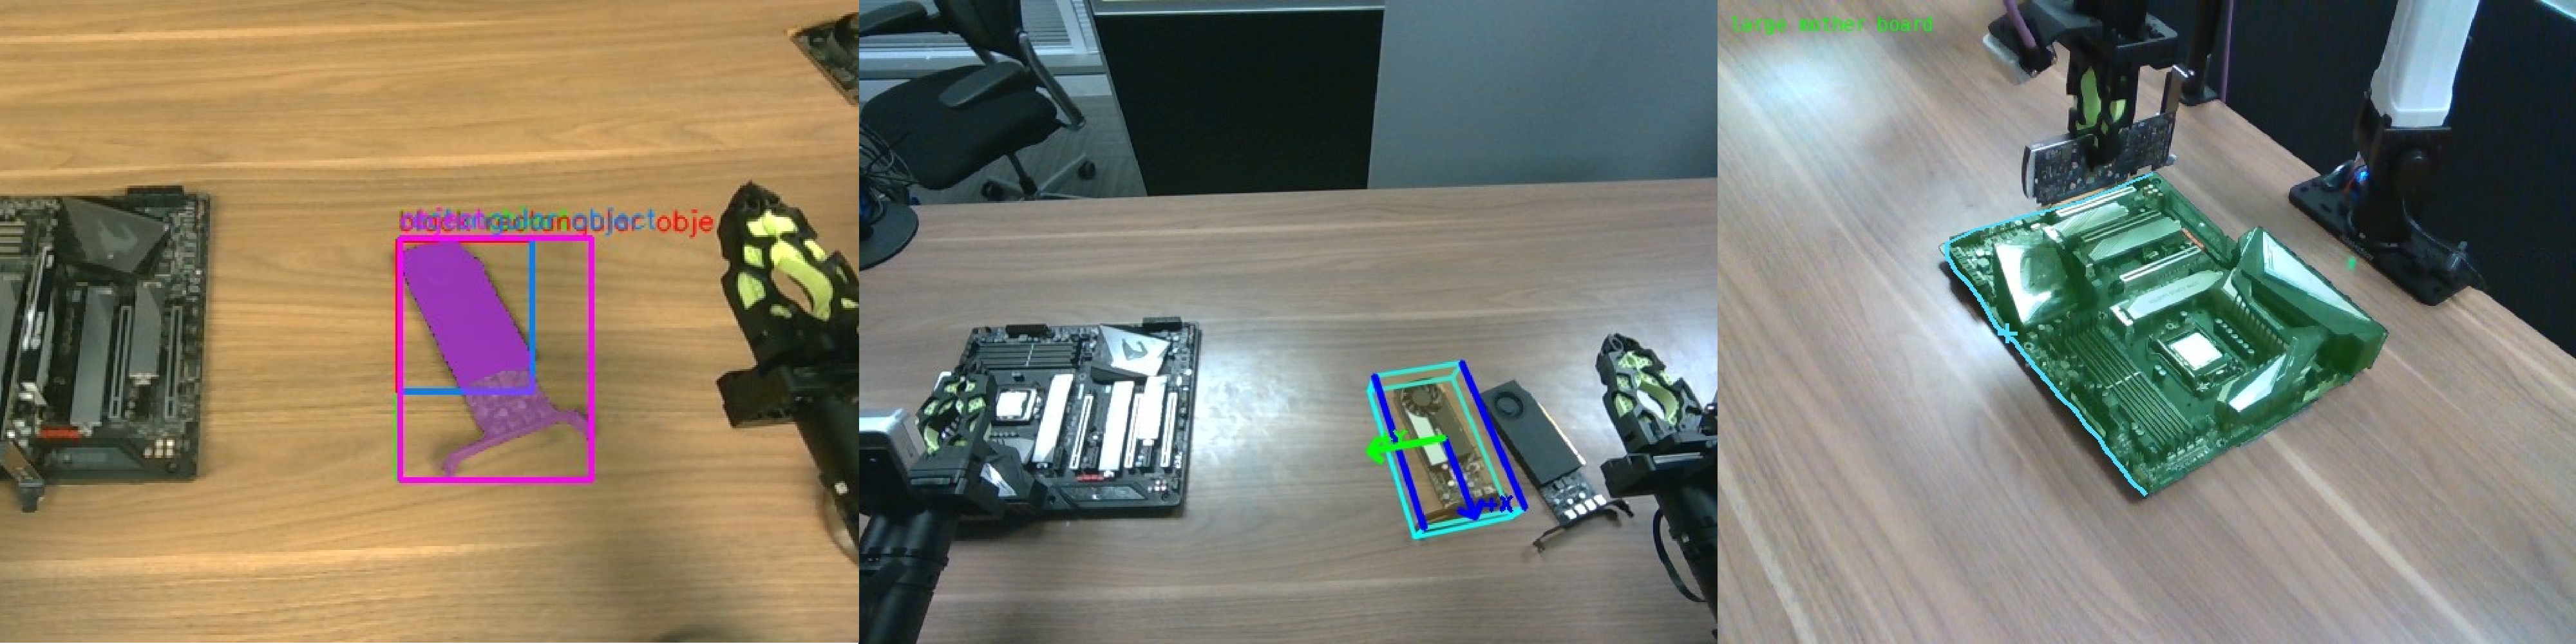
\includegraphics[width=0.9\linewidth]{corl_2026_template_submission/figures/example/gpu_gofe_tools.pdf}
    \caption{Visual tools for GPU insertion. Agent-written auxiliary detection tools for GPU localization via SAM3 and depth estimation.}
    \label{fig:visual_tools_gpu_insertion}
\end{figure}




\subsection{Autoresearch-driven Reward Design} 
Autoresearch can be applied to automate the design of reward functions. This procedure requires human effort in only two steps: first, collect a few minutes of representative success and failure demonstrations; second, specify the reward design requirements, including target precision, recall, and inference latency. 

As an example, we assign the agent to build a visual reward function that detects whether a zip tie is fastened. For evaluation, we record a few minutes of labeled success and failure snapshots of zip tie fastening as a sandboxed held-out evaluation set—the agent may study failures, but cannot train on the test set or alter metric computation. The agent autonomously probes the SAM3 API via prompt search, tunes cropping and depth thresholds to suppress background noise, and meets the 150 ms latency budget by converting to ONNX, compiling the computation graph for simultaneous multi-object forward passes. The decision-making logic converges on the two-view geometric test, illustrated in \Cref{fig:zip_tie_reward}. A simplified implementation is provided in \Cref{fig:reward_impl}.

Autoresearch is not limited to visual rewards; the coding agent can compose hybrid reward functions that fuse multiple sensing modalities, including proprioception and end-effector force estimates. As an example, \Cref{fig:pin_insertion_reward} illustrates an autonomously designed reward for pin insertion that combines visual alignment, depth of insertion, and contact force signals.

\captionof{codesnippet}{\textbf{Dual-View Zip Tie Verification.} Combines the top and right camera views in a geometric test of whether the zip-tie strap passes through the head, guarding against single-view false positives.}
\label{fig:reward_impl}
\begin{appendixcode}{python}
def get_reward_from_top_right_cam(rgb_t, rgb_r):
    dets = segment_zip_tie_views(rgb_t, rgb_r, threshold=sam3_score_threshold)
    strap = union([d["mask"] for d in top2_by_score(dets["top"]["strap"])])
    head = top1_by_score(dets["top"]["head"])["mask"]
    strap = binary_dilation(strap, iterations=top_dilate)
    head = binary_dilation(head, iterations=top_dilate)
    overlap = (strap & head).sum() / head.sum()
    protrude = strap[:, :head_left_x(head)].sum() / head.sum()
    top_ok = overlap >= top_inter_frac and protrude >= top_left_mult

    right = binary_dilation(dets["right"]["strap"]["mask"], iterations=right_dilate)
    head_box = bbox_shrunk(dets["right"]["head"], frac=right_shrunk_frac)
    labeled, n_comp = label(right)
    if n_comp == 2:
        right = right | connect_components(labeled)
    right_ok = n_comp in (1, 2) and (right & head_box).any()
    return top_ok and right_ok
\end{appendixcode}





\begin{figure}[H]
    \centering
    \includegraphics[width=0.95\linewidth]{corl_2026_template_submission//figures/agent-generate-env.pdf}
    \caption{Reward function for pin insertion.
    The agent proposes a hybrid verification strategy fusing visual alignment of the
    pin tip to the hole, insertion depth from proprioception signals, and end-effector torque detection.}
    \label{fig:pin_insertion_reward}
\end{figure}


% breakable typewriter identifier for long API names
\newcommand{\api}[1]{\texttt{\detokenize{#1}}}




\section{Robot System Setup}
\label{app:robot-system}

\subsection{Fleet Architecture}
\label{app:fleet}
Our physical infrastructure is a fleet of \textbf{eight bimanual robot stations}, operated in a decentralized manner. Each station owns its robot arms and cameras, compute, and its own coding agent. Hardware-control requests from each station's agent are routed through a local FastAPI server. Coordination across stations is mediated entirely through \textbf{Git}: rather than streaming state to a central server, stations share code, configurations, tools, and results by pushing to and pulling from a common repository, so that improvements discovered on one station propagate to the rest through ordinary version control. Because all coordination flows through Git, agents can borrow ideas from one another: they freely merge changes from other branches or cherry-pick individual commits, selectively adopting promising approaches and results discovered at other stations. This keeps the fleet loosely coupled and fault-tolerant, since stations run, fail, and recover independently, while the shared Git history serves as the single source of truth for what each station has tried and learned.
\ifdefined\nvidiareleaseomitappendixfleet
\else
\begin{figure}[h]
\centering
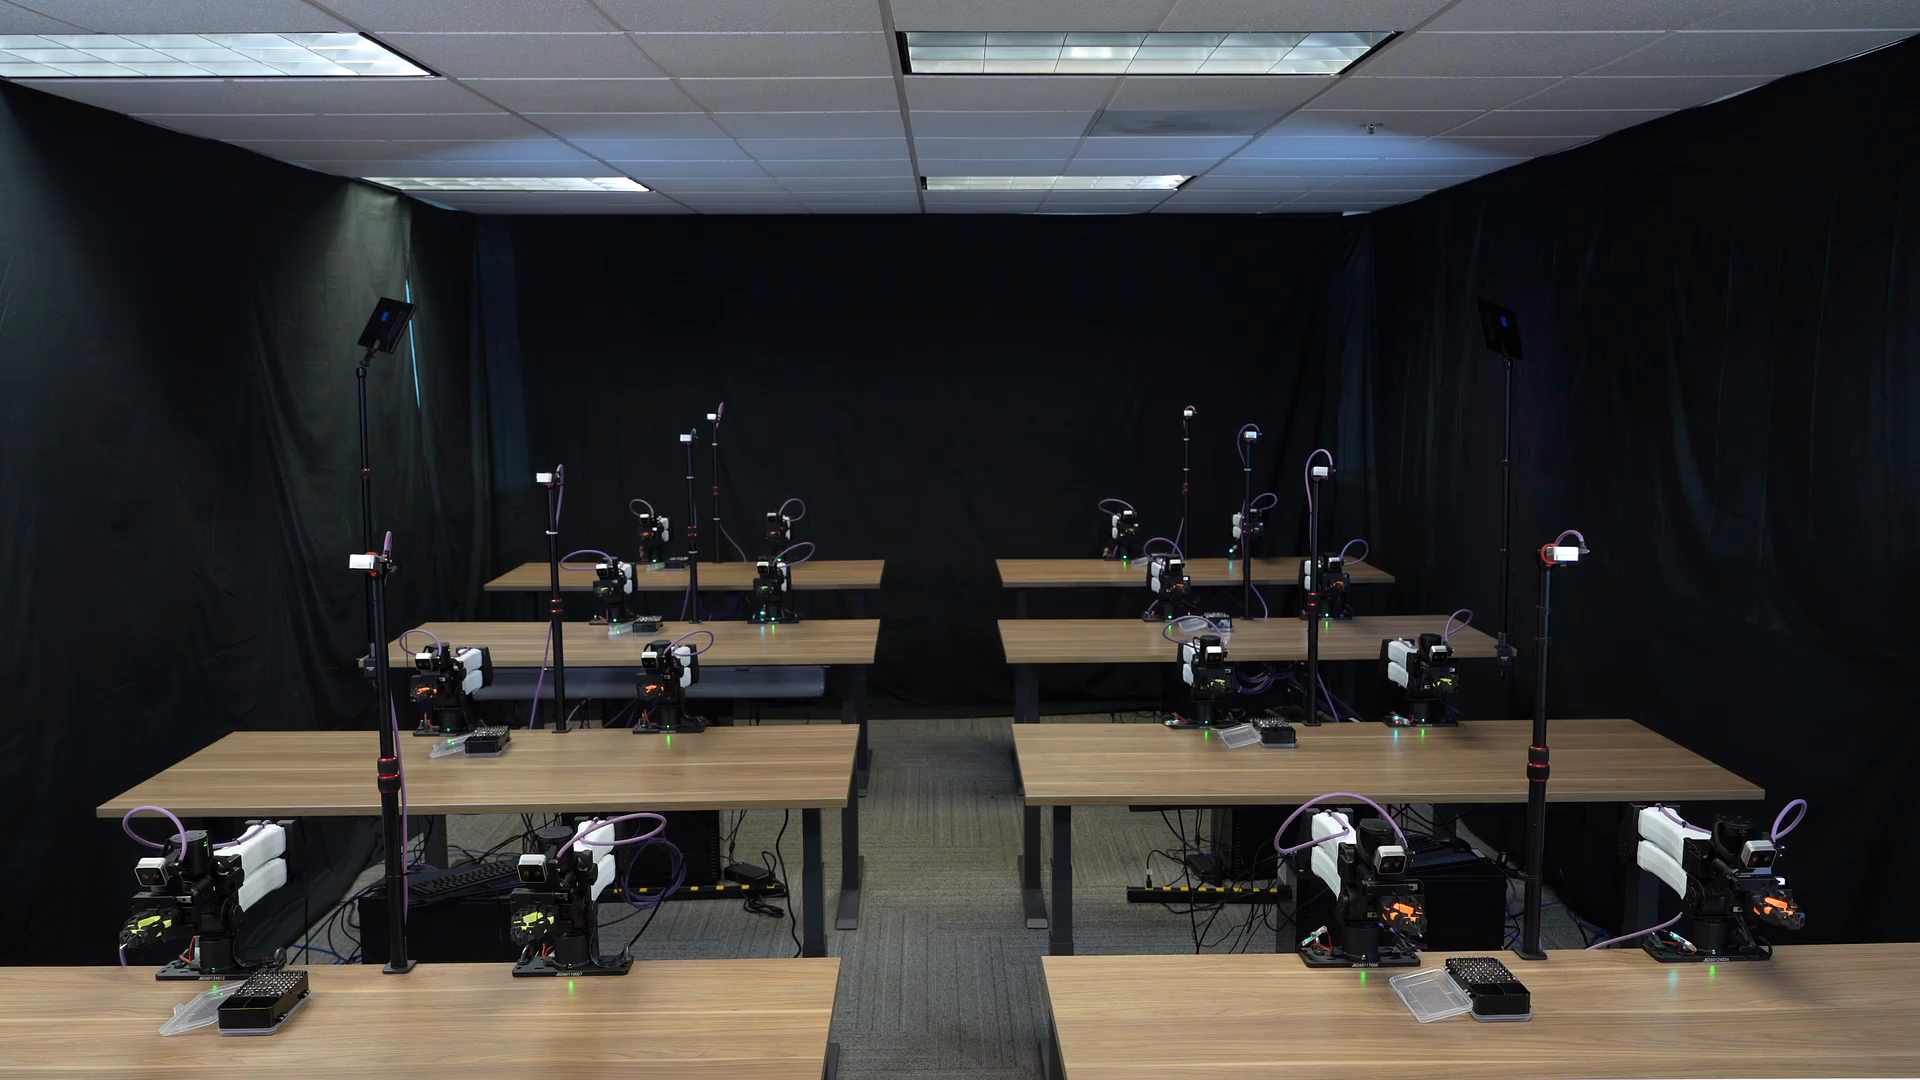
\includegraphics[width=\linewidth, trim=0 0 0 265, clip]{figures/fleet.png}
\caption{The fleet of eight bimanual YAM robot stations. Each station owns its robot hardware, compute, and coding agent.}
\label{fig:fleet}
\end{figure}
\fi

\paragraph{Control endpoints.}
The FastAPI server exposes a small set of endpoints through which the agent drives data collection and execution: \texttt{/start} begins a rollout on the real hardware, \texttt{/restart} allocates a fresh rollout buffer directory, and \texttt{/home} returns the arms to the home configuration. The \texttt{/restart} endpoint keeps successive rollouts separate and individually addressable, so that the data from different hypotheses or experiments is never mixed together: each rollout is written to its own directory, and the agent can attribute outcomes to the specific change it was testing. These endpoints are shared across all of our tasks. The Push-T task additionally exposes \texttt{/avoid} and \texttt{/resume} endpoints to handle occlusion: \texttt{/avoid} backs the arm out of the top-camera frame so it no longer occludes the scene, and \texttt{/resume} returns the arm to its original position to continue manipulation.

\paragraph{Agent sandbox and context.}
Each station's coding agent operates within a sandbox scoped to a single autoresearch repository. Within this sandbox the agent runs with elevated autonomy: action-level permission prompts are bypassed, so it can execute commands without per-step human approval, and it is granted unrestricted internet access. The agent is provided with the complete set of robot data collected during the current autoresearch session, and is free to make full use of all available information in pursuit of its objective. For ordinary fresh sessions, raw repository state, rollout data, checkpoints, and transient logs from prior sessions are pruned before initialization, so that the agent starts from a clean, isolated workspace. For transfer experiments, such as initializing GPU insertion after pin insertion, the agent is instead given an explicit markdown summary distilled from the previous pin-insertion autoresearch session; raw trajectories, hidden logs, and checkpoints are still removed, so transfer occurs through the written summary rather than through unbounded access to prior session state. The prompt given to each station's agent is shown in \Cref{fig:autoresearch-prompt}.

\begin{figure}[t]
\begin{minted}[fontsize=\small, frame=lines, framesep=2mm, breaklines=true]{text}
/goal Achieve a 100% success rate over each window of 50 consecutive
episodes. Read @auto_research.md and fan out a subagent team to study
different algorithms (RL, BC, hybrid). You may reuse checkpoints or data
buffers across hypotheses. Create your own branch from autorl following the
instructions. Do not directly work on or push to autorl. You must actively
monitor other branches and commits from origin that branched off autorl to
leverage knowledge from those branches. You must actively push your branch to
contribute to the repo and pull from origin. Collaborate with other agents
via Git.
\end{minted}
\caption{The autoresearch prompt provided to each station's coding agent.}
\label{fig:autoresearch-prompt}
\end{figure}

\subsection{Station Hardware}
\label{app:station}
All 8 stations are hardware-identical. Each station comprises two YAM (Yet Another Manipulator) arms from I2RT in a fixed bimanual configuration, a set of cameras, and a single workstation that runs the FastAPI server, policy inference, and the station's agent.

\paragraph{Manipulators and actuation.}
Each arm is a 6-DoF manipulator equipped with a 1-DoF parallel-jaw gripper, giving seven actuated joints per arm and fourteen across the bimanual pair. All joints are driven by brushless actuators over a CAN bus. The six arm joints are run under PD control with gravity compensation, while the gripper is run in a force-limited mode that bounds grip force directly (\Cref{app:lowlevel}); we exploit this gripper-level force limiting both for robust grasping and for safe, unattended operation across the fleet.

\paragraph{Compute.}
Each station runs on a single workstation whose specifications are listed in \Cref{tab:compute}. All policy inference and on-station computation run on this single GPU, with no shared cluster or off-station compute.

\begin{table}[h]
\centering
\caption{Per-station compute specifications.}
\label{tab:compute}
\begin{tabular}{ll}
\toprule
Component & Specification \\
\midrule
GPU       & 1$\times$ NVIDIA RTX 5090, 32\,GB \\
CPU       & Intel Core Ultra 9 285K, 24 cores \\
RAM       & 128\,GB \\
OS        & Ubuntu 22.04 LTS \\
GPU stack & NVIDIA driver 595.58.03, CUDA 13.2 \\
\bottomrule
\end{tabular}
\end{table}

\paragraph{Perception.}
Unless noted otherwise, perception uses Intel RealSense \textbf{D405} cameras: one top-down camera viewing the workspace and two wrist-mounted cameras, one per arm, that provide close-range views of the grasped object and the contact region. One task also uses a side-mounted RealSense \textbf{D435i} for a wider third-person view (\Cref{app:gpu-insert}). The policy runs at \textbf{30\,Hz}, and its action targets are tracked by the low-level joint controllers described below, which run at \textbf{100\,Hz} over the CAN bus. We additionally use \textbf{Viser} for real-time, browser-based 3D visualization of robot state, camera frames, and target poses, which supports monitoring of autonomous runs, calibration debugging, and episode inspection.

\subsection{Low-Level Control}
\label{app:lowlevel}
Policy actions are inferred at \textbf{30\,Hz}, and each action target is tracked by the low-level joint controllers running at \textbf{100\,Hz} over the CAN bus. The two joint groups are controlled differently. The six arm joints use \textbf{PD control with gravity compensation}, which tracks the commanded joint targets while the feedforward gravity term offloads the static load so the PD gains only need to handle the residual error.

\vspace{0.5cm}
The 1-DoF gripper runs as a \textbf{torque-limiting compliant grasp}: instead of closing to a rigid target width, the gripper applies a bounded grip force set by a commanded torque limit. This force limiting is the key to robust and safe grasping. Because the fingers settle around the object at a bounded force rather than driving to a fixed position, the grasp accommodates variation in object pose and size and is robust to perception and placement error. The same bound caps the force the system can exert during grasping, contact, and insertion, preventing damage to the gripper, the manipulated parts, and the fixtures when an attempt is misaligned or fails. Because the fleet operates autonomously and unattended across all 8 stations, this bounded-force behavior is essential: a bad contact results in a safe stall rather than a hardware-damaging push, with no human in the loop to intervene.

\subsection{Per-Task Configuration}
\label{app:gpu-insert}

\begin{figure}[h]
\centering
\begin{minipage}[t]{0.48\linewidth}
\centering
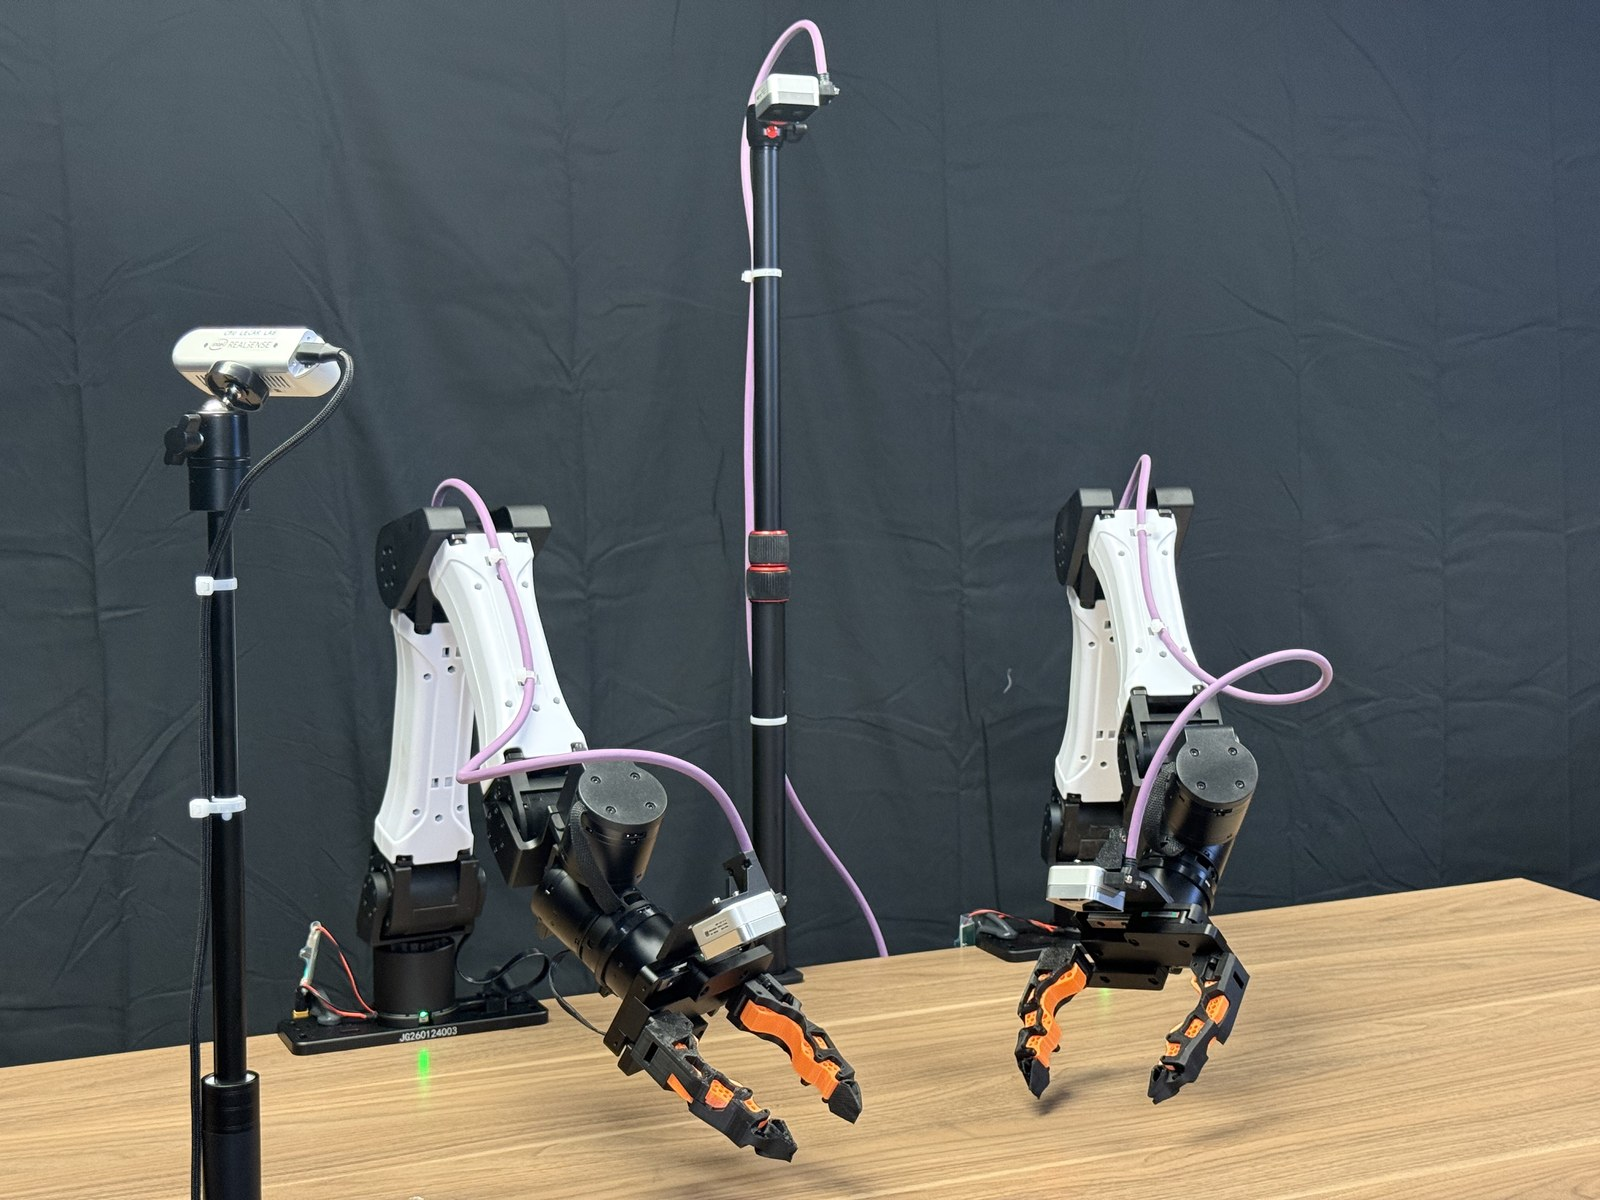
\includegraphics[width=\linewidth]{figures/four_camera_setup.jpg}
\subcaption{Four-camera setup (GPU insertion).}
\label{fig:four-cam}
\end{minipage}\hfill
\begin{minipage}[t]{0.48\linewidth}
\centering
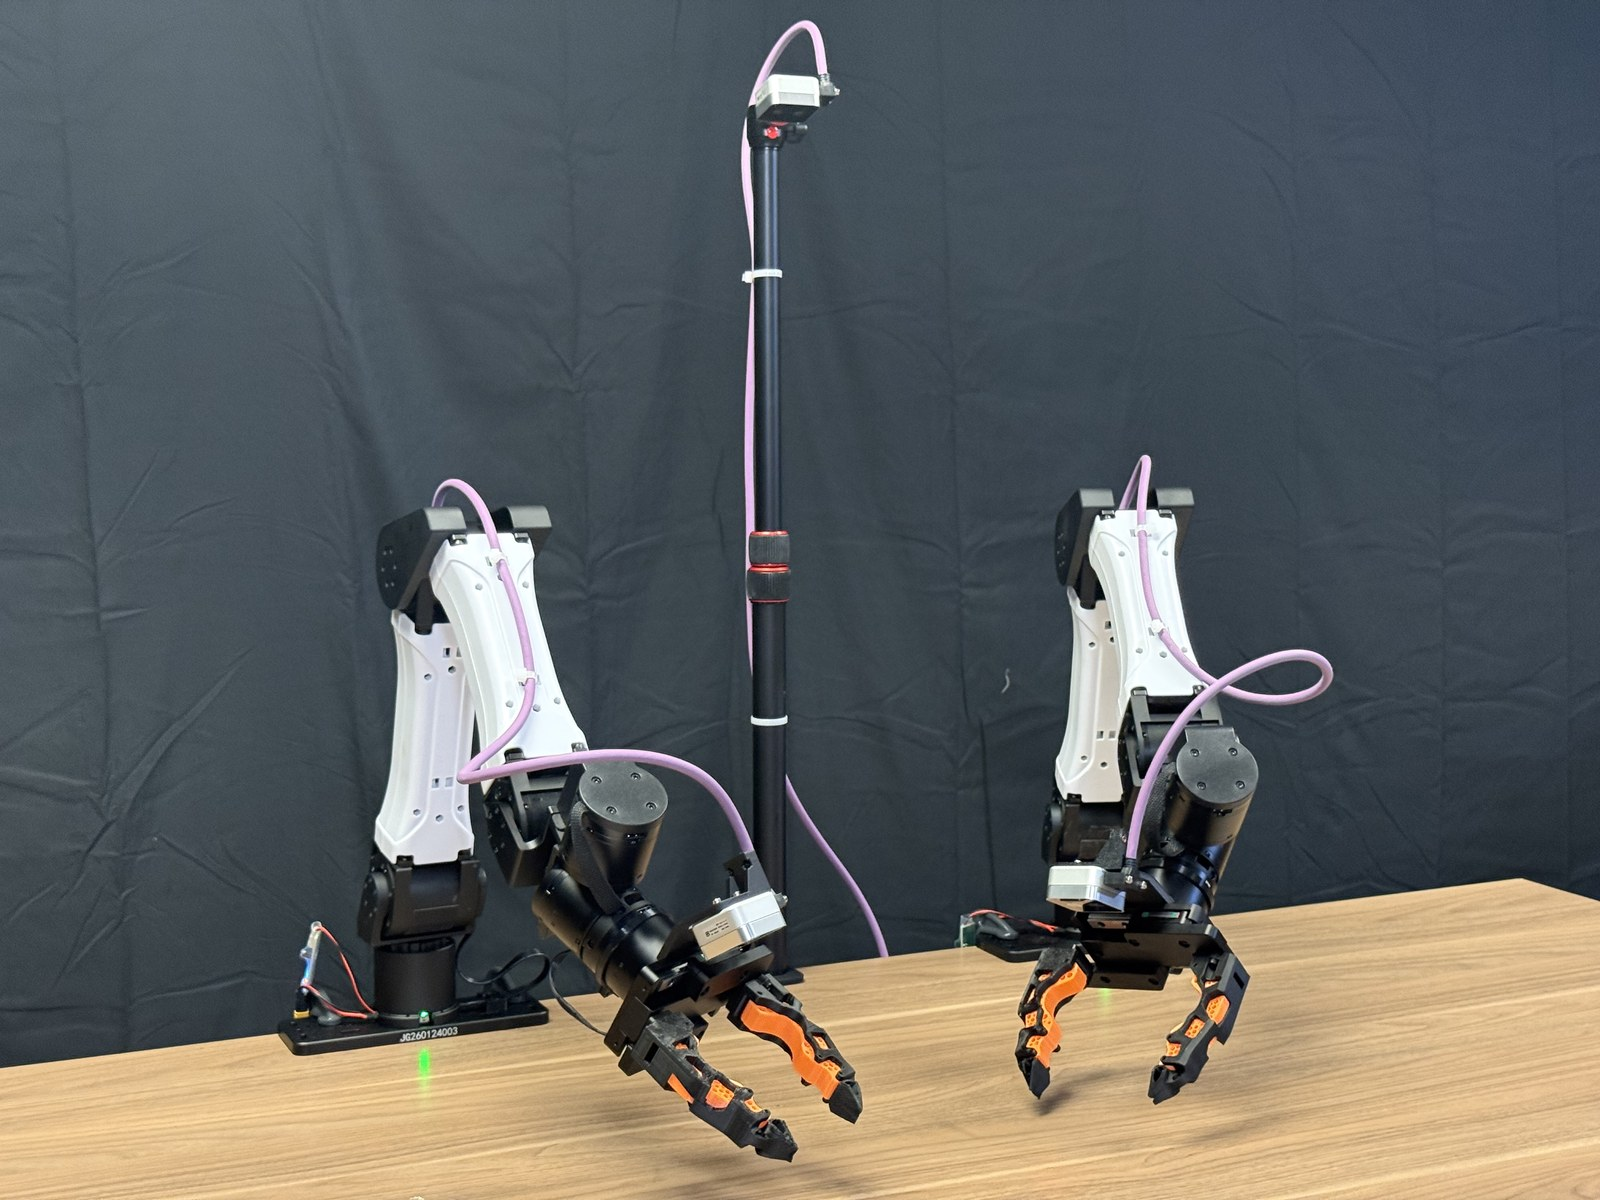
\includegraphics[width=\linewidth]{figures/three_camera_setup.jpg}
\subcaption{Three-camera setup (pin insertion, Push-T, zip tie).}
\label{fig:three-cam}
\end{minipage}
\caption{Per-station camera configurations. All tasks use one top-down camera and two wrist-mounted cameras, all RealSense D405. The GPU insertion task in \Cref{fig:four-cam} additionally uses a side-mounted RealSense D435i on the left pole for a wider third-person view of the slot; the remaining tasks use the three-camera setup in \Cref{fig:three-cam}.}
\label{fig:camera-setups}
\end{figure}

The four tasks share the station hardware and the 30\,Hz policy loop above, and differ only in minor details of their camera and control configuration. As shown in \Cref{fig:camera-setups}, all four use one top-down camera and two wrist cameras, all RealSense D405; the GPU insertion task additionally uses a side-mounted RealSense D435i for a wider third-person view of the slot.


\subsection{Real-World RL System Integration}
We integrated the PLD-RL pipeline~\cite{pld} to provide a controlled sandbox for the coding agent to conduct algorithm auto-research with online data collection. The infrastructure is developed following the asynchronous design of SERL~\citep{luo2024serl, luo2025precise}. We implement it as a three-tier distributed system that decouples robot interaction, policy learning, and inference across separate processes. The deployment layer runs on a robot-adjacent control machine and is responsible for hardware orchestration, episode recording, and human-in-the-loop teleoperation. The second tier, learner, runs on a GPU host and trains an RL agent (actor \& critic) with pixel observations encoded through a pre-trained visual backbone. The third tier, actor, exposes a Portal/ZMQ msgpack-compatible endpoint, so that the controller can request actions through a uniform protocol shared with scripted and teleoperated control modes.


Data flow between the deployment layer and the learner is mediated by a deliberately loose disk-based contract. The deployment layer serializes each episode as a per-step observation tensor and synchronized camera streams (.mp4) into a rollout-buffer directory, accompanied by a per-step action label identifying the action source (rl, human, etc.). Meanwhile, a daemon thread (\textit{DiskBufferIngestor}) polls this directory periodically, parses newly finalized episodes, and routes transitions by action-source label following the RLPD-style data-mixing protocol~\citep{rlpd}: RL-generated transitions populate the online replay buffer, while human and manual transitions populate a separate demonstration buffer that is mixed into each training batch. This design is flexible for mixing data from different sources.

\subsection{Idea Tree for Pin Insertion}
\label{app:idea-tree-pin}
\Cref{fig:idea-tree-pin} visualizes an agent-team autoresearch run on the pin
insertion task as an idea tree (top) paired with its hill-climbing curve (bottom).
Each node $\mathrm{I}k$ is an idea explored by the team; ideas that are related are
connected by a horizontal line, and each new lane corresponds to a new branch of ideas.
Solid green nodes mark ideas that improved the team-average best success rate, while
hollow nodes were evaluated but yielded no gain. The thick black line traces the lineage
of the highest-scoring idea. Circled nodes are highlighted ideas that are also annotated
on the hill-climbing curve below, to which they are connected by dashed lines. The bottom
panel reports the team-average best success rate as a function of research wall-clock time, sharing the time axis of the tree above. As the agents collaborate through Git,
a few high-impact ideas account for most of the progress---most notably BC regularization
(I37, $+10.8$\,pp)---while later ideas such as batch-size tuning (I66, $+0.9$\,pp) and
controller compensation (I76, $+1.3$\,pp) contribute smaller, incremental refinements as
the success rate approaches $100\%$.

\begin{figure*}[t]
\centering
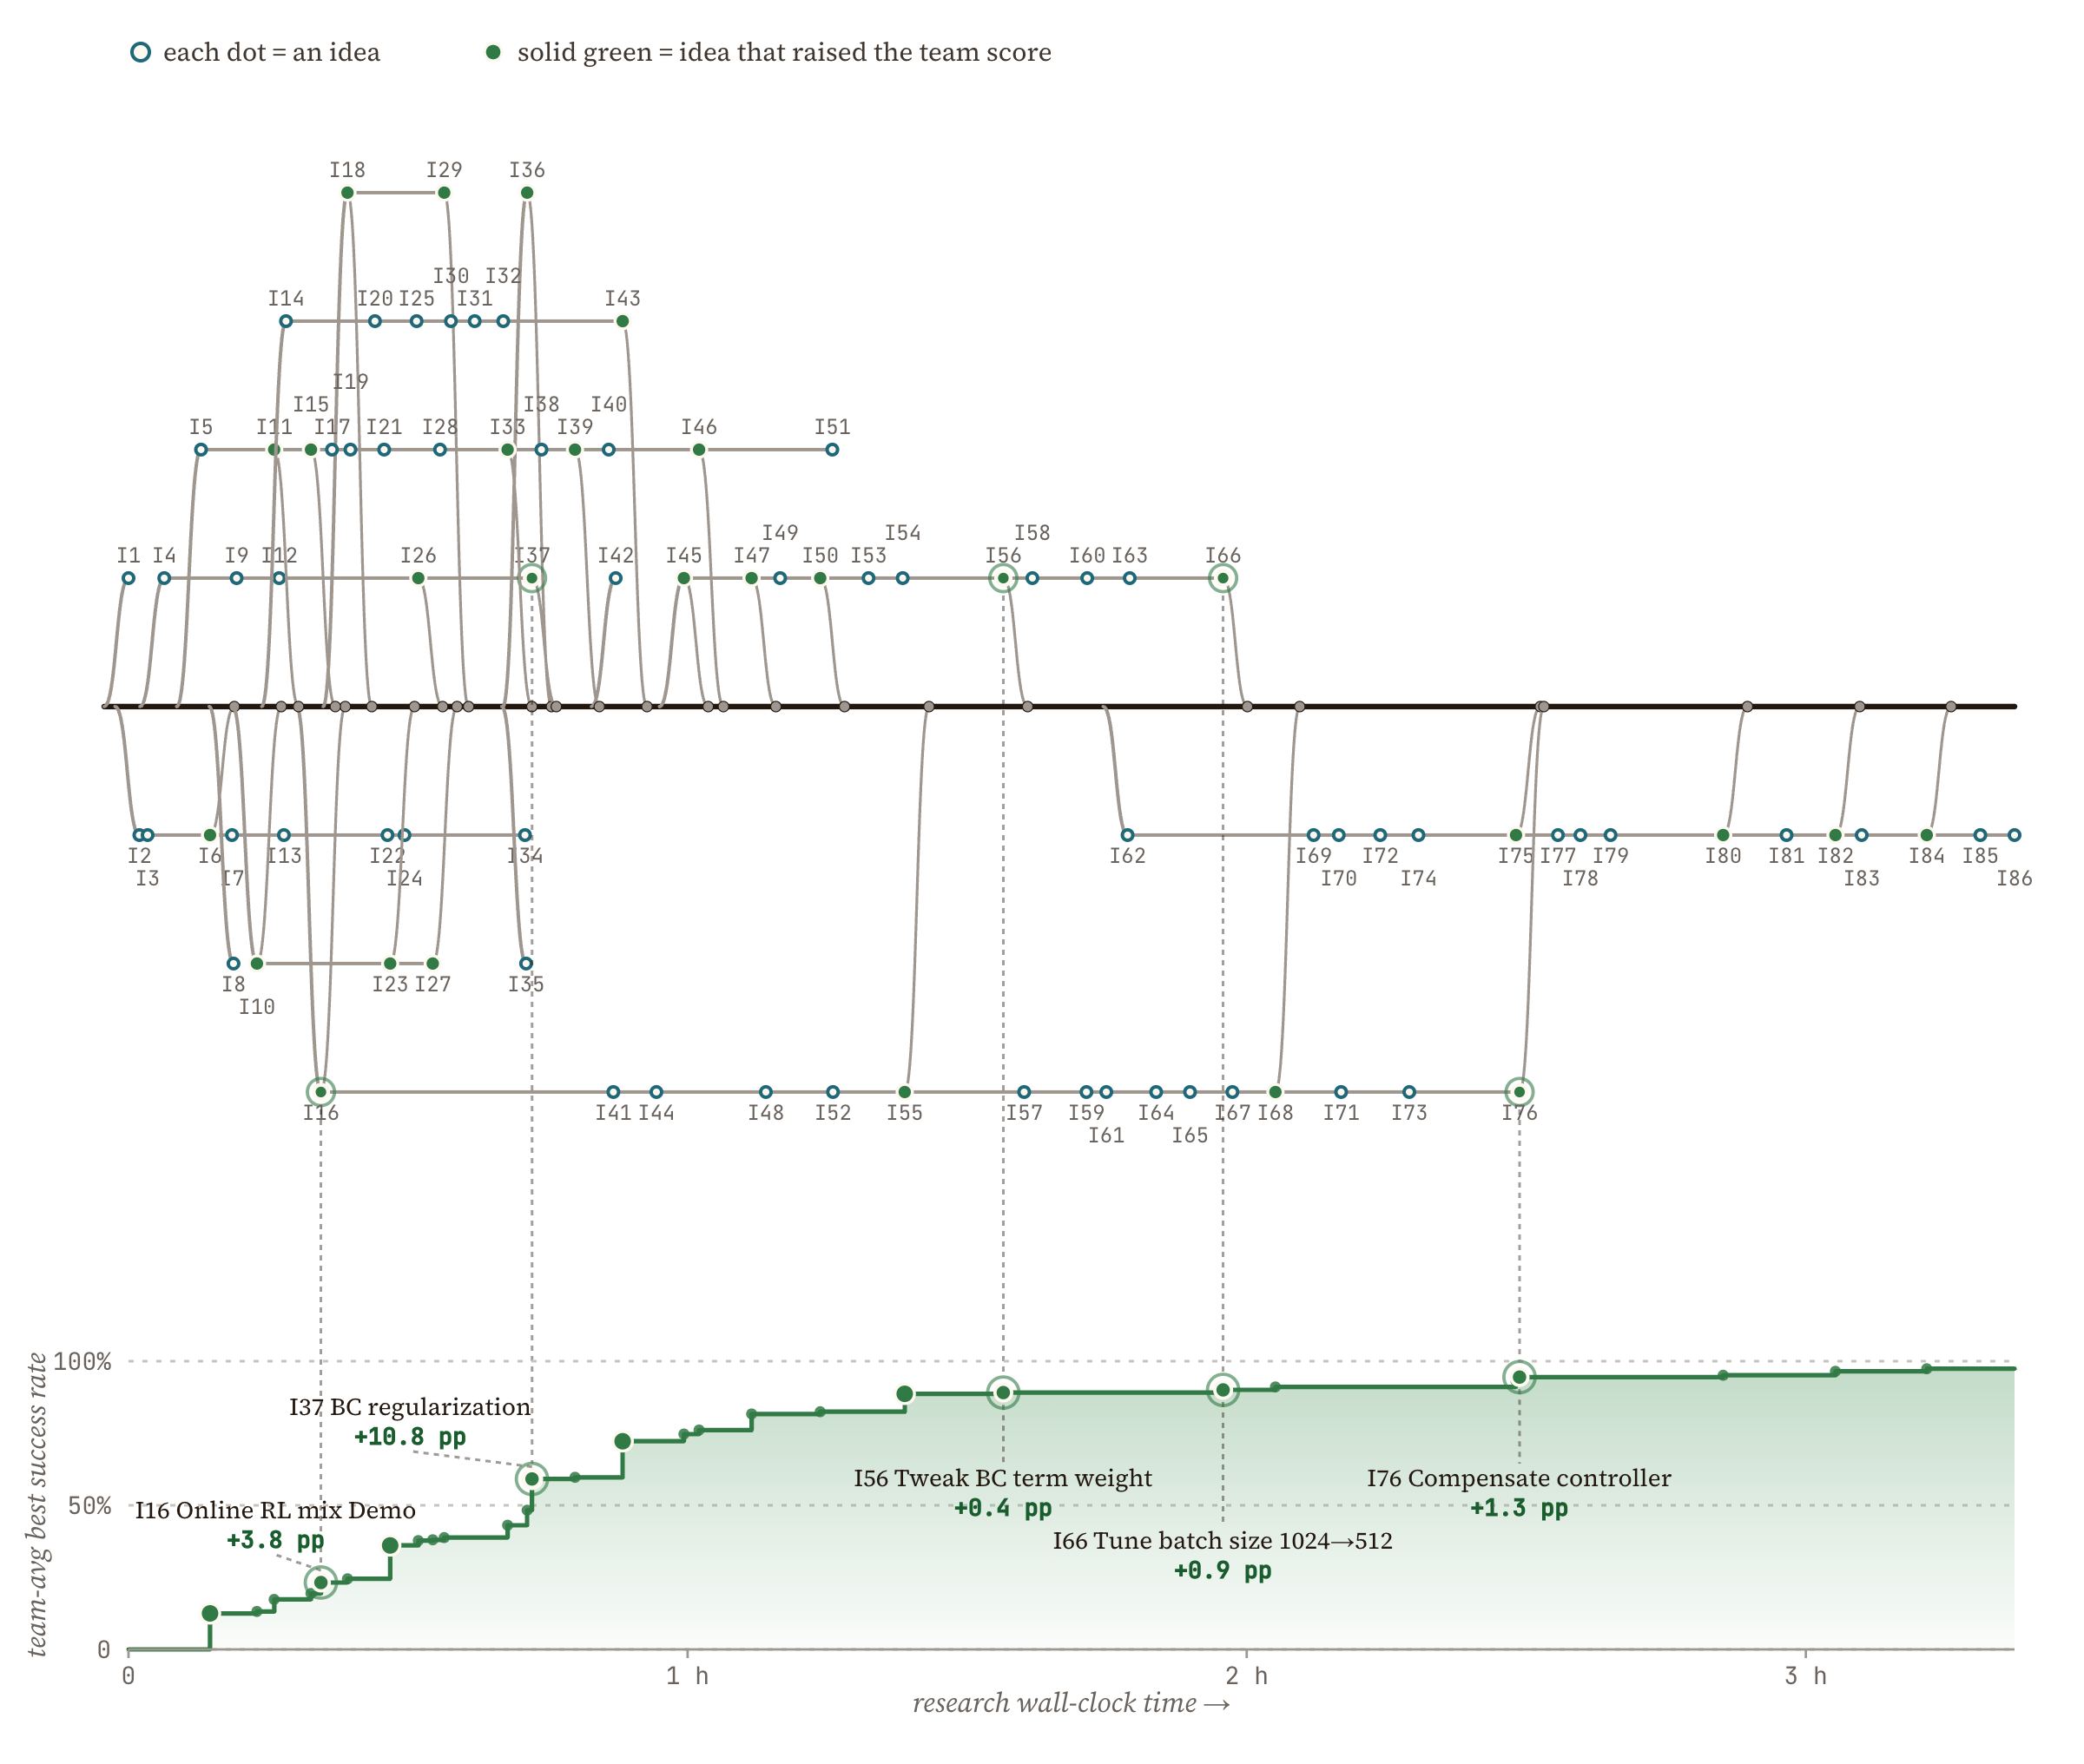
\includegraphics[width=\linewidth]{figures/idea_tree_pin.png}
\caption{\textbf{Idea tree and hill-climbing progress for the pin insertion task.}
\emph{Top:} the agent's idea tree, where each node $\mathrm{I}k$ is a proposed idea and
each new lane is a new idea branch. Two nodes joined by a horizontal line are related
ideas. Solid green nodes improved the team-average best success rate; hollow nodes were
evaluated but yielded no gain. The thick black line traces the lineage of the
highest-scoring idea, and circled nodes are highlighted ideas linked by dashed lines to
their milestones below. \emph{Bottom:} the team-average best success rate over research
wall-clock time, sharing the time axis of the tree. Annotated milestones report each
highlighted idea's improvement in percentage points (pp).}
\label{fig:idea-tree-pin}
\end{figure*}

\section{Physical Autoresearch: Ablation Studies}

\subsection{Experimental Setup}
We constructed a simplified real-world Push-T environment, \texttt{pusht-simple}, for controlled ablations of the autoresearch agent. The task preserves the core visual servoing and contact-planning structure of Push-T while reducing episode length and setup variability, making it suitable for repeated comparisons across model, harness, and visual-grounding conditions. Compared with the Push-T task in the main paper, this variant uses a relaxed success boundary so that ablations can focus on controller discovery rather than rare terminal precision. An episode is counted as successful when the pushed T block reaches the target region within the prescribed translational tolerance and its orientation is within $10^\circ$ of the goal orientation. Operationally, the agent must write a controller that rotates the T block by approximately $180^\circ$ and places it inside the enlarged success region.


\subsection{Token Utilization}

\begin{figure}
    \centering
    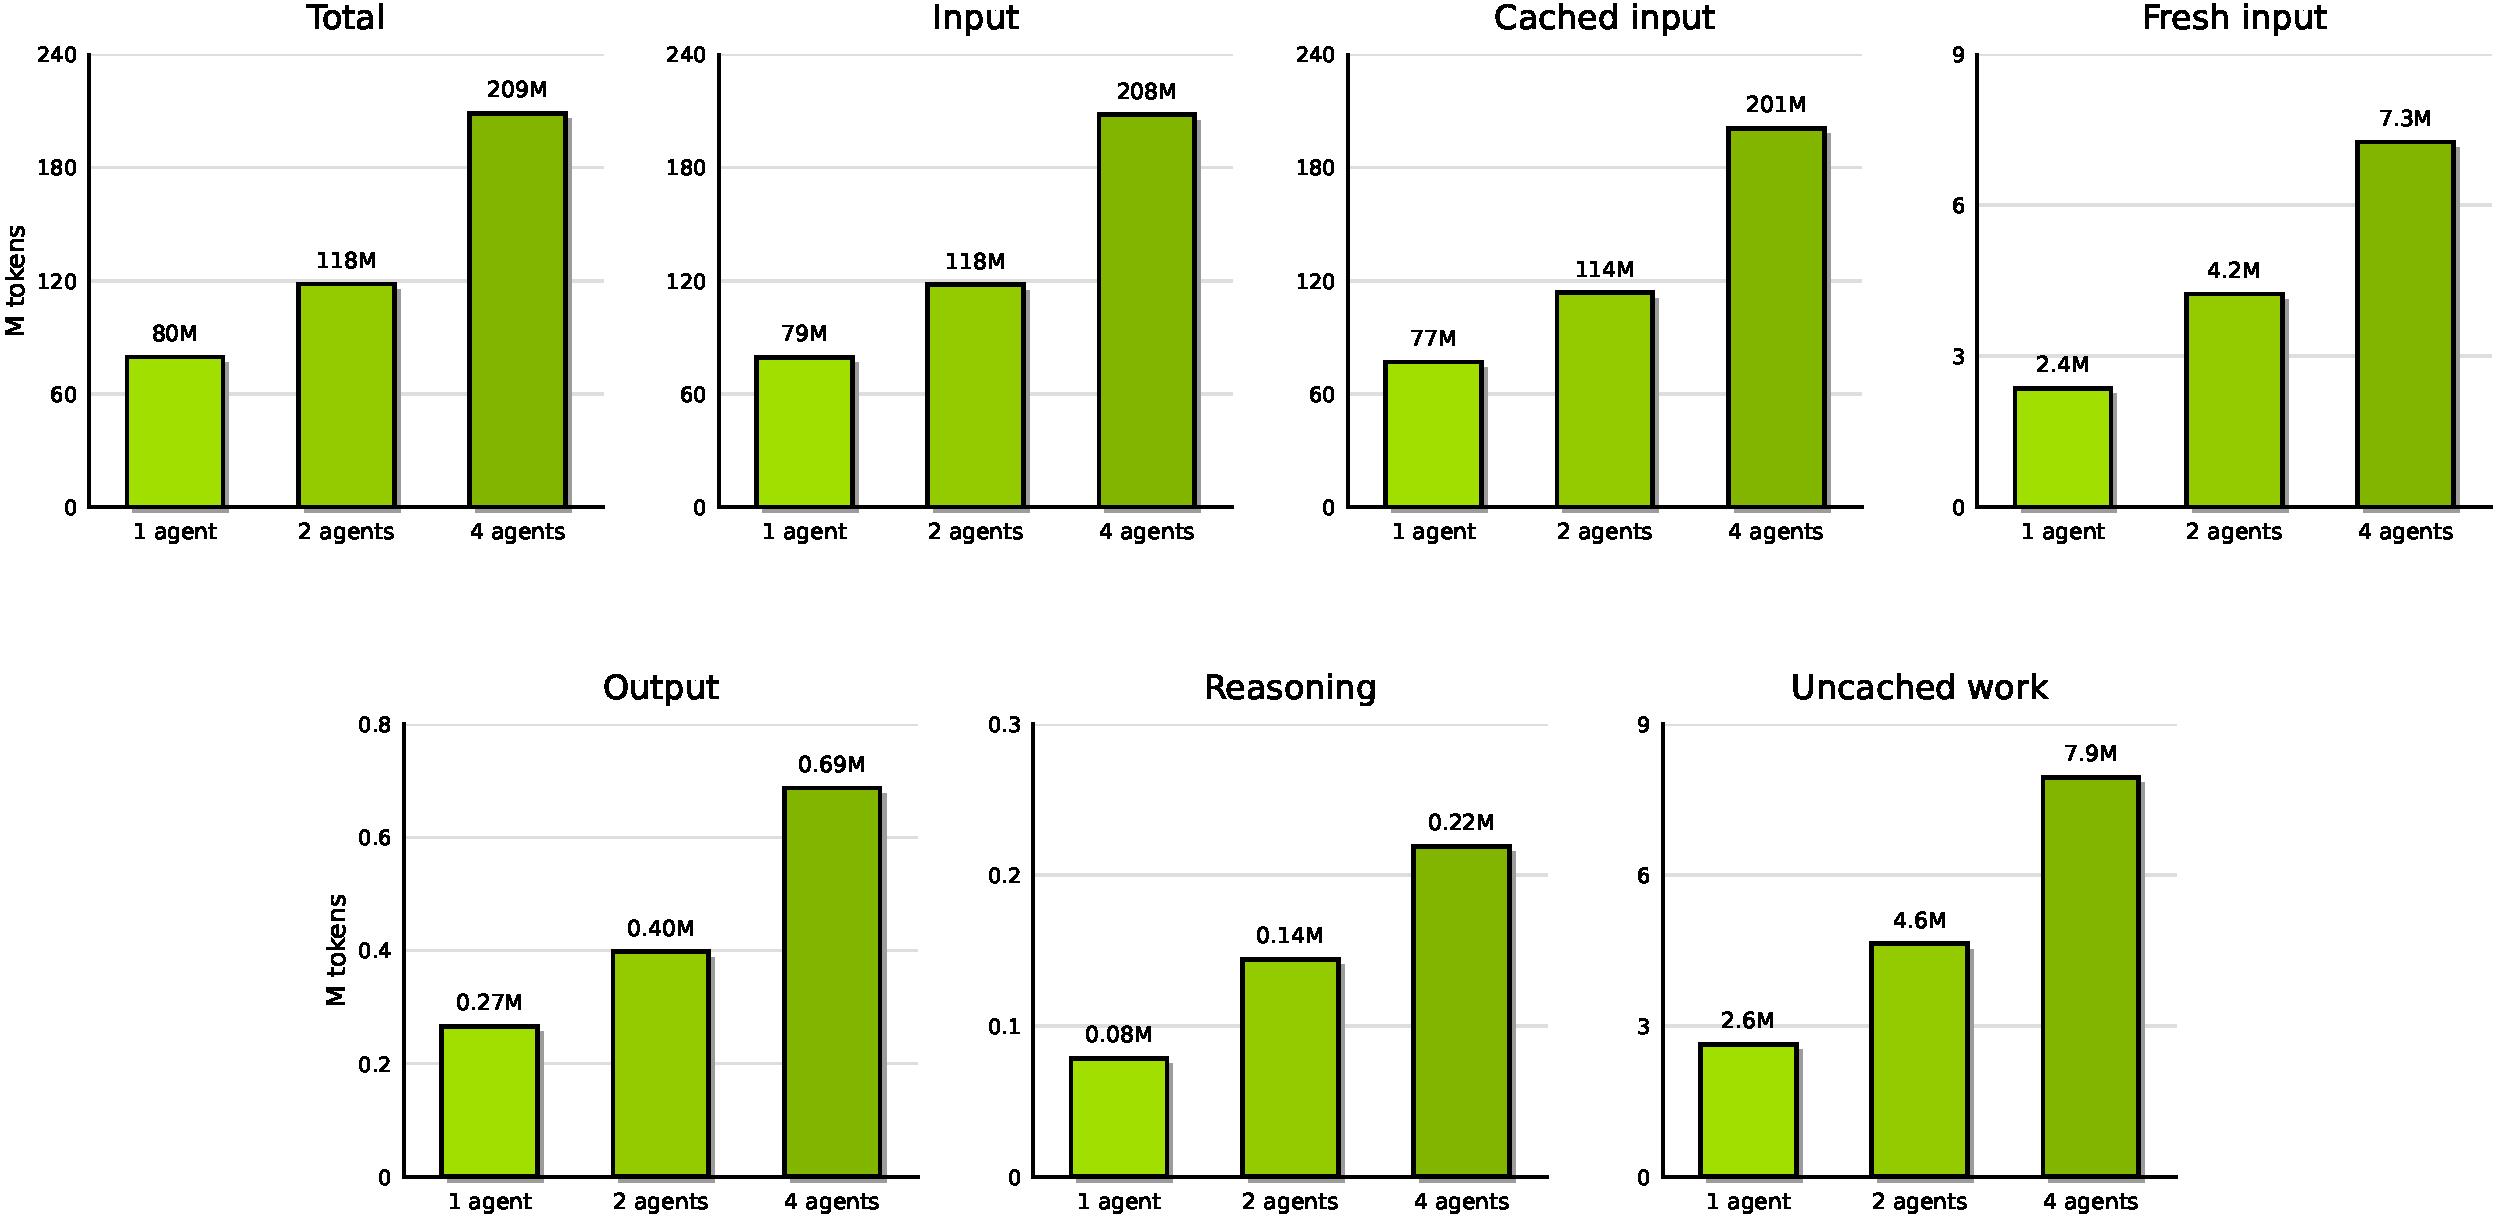
\includegraphics[width=1\linewidth]{corl_2026_template_submission//figures/codex_token_scaling_7panel.pdf}
    \caption{Token-utilization breakdown for Codex agents on the simplified real-world Push-T task. Each panel reports a different view of token consumption over the autoresearch process, separating prompt/input, generated/output, and cached-context usage where available. The figure complements the aggregate MTU analysis in the main paper by showing how token demand is distributed across planning, code editing, log inspection, and repeated policy-evaluation iterations.}
    \label{fig:token_utilization_breakdown}
\end{figure}

In the main paper, we summarize token scaling by aggregating input and output tokens. Because input, output, and cached tokens differ in cost, latency, and the type of agent activity they reflect, we additionally report token usage by category. This breakdown clarifies how much of the autoresearch budget is spent on context ingestion, code and plan generation, and reuse of cached interaction history. For a more detailed qualitative analysis, we visualize total token usage, input token usage, cached input token usage, fresh input token usage, output token usage, and reasoning token usage.

\subsection{Native Vision Capability}

\begin{figure}
    \centering
    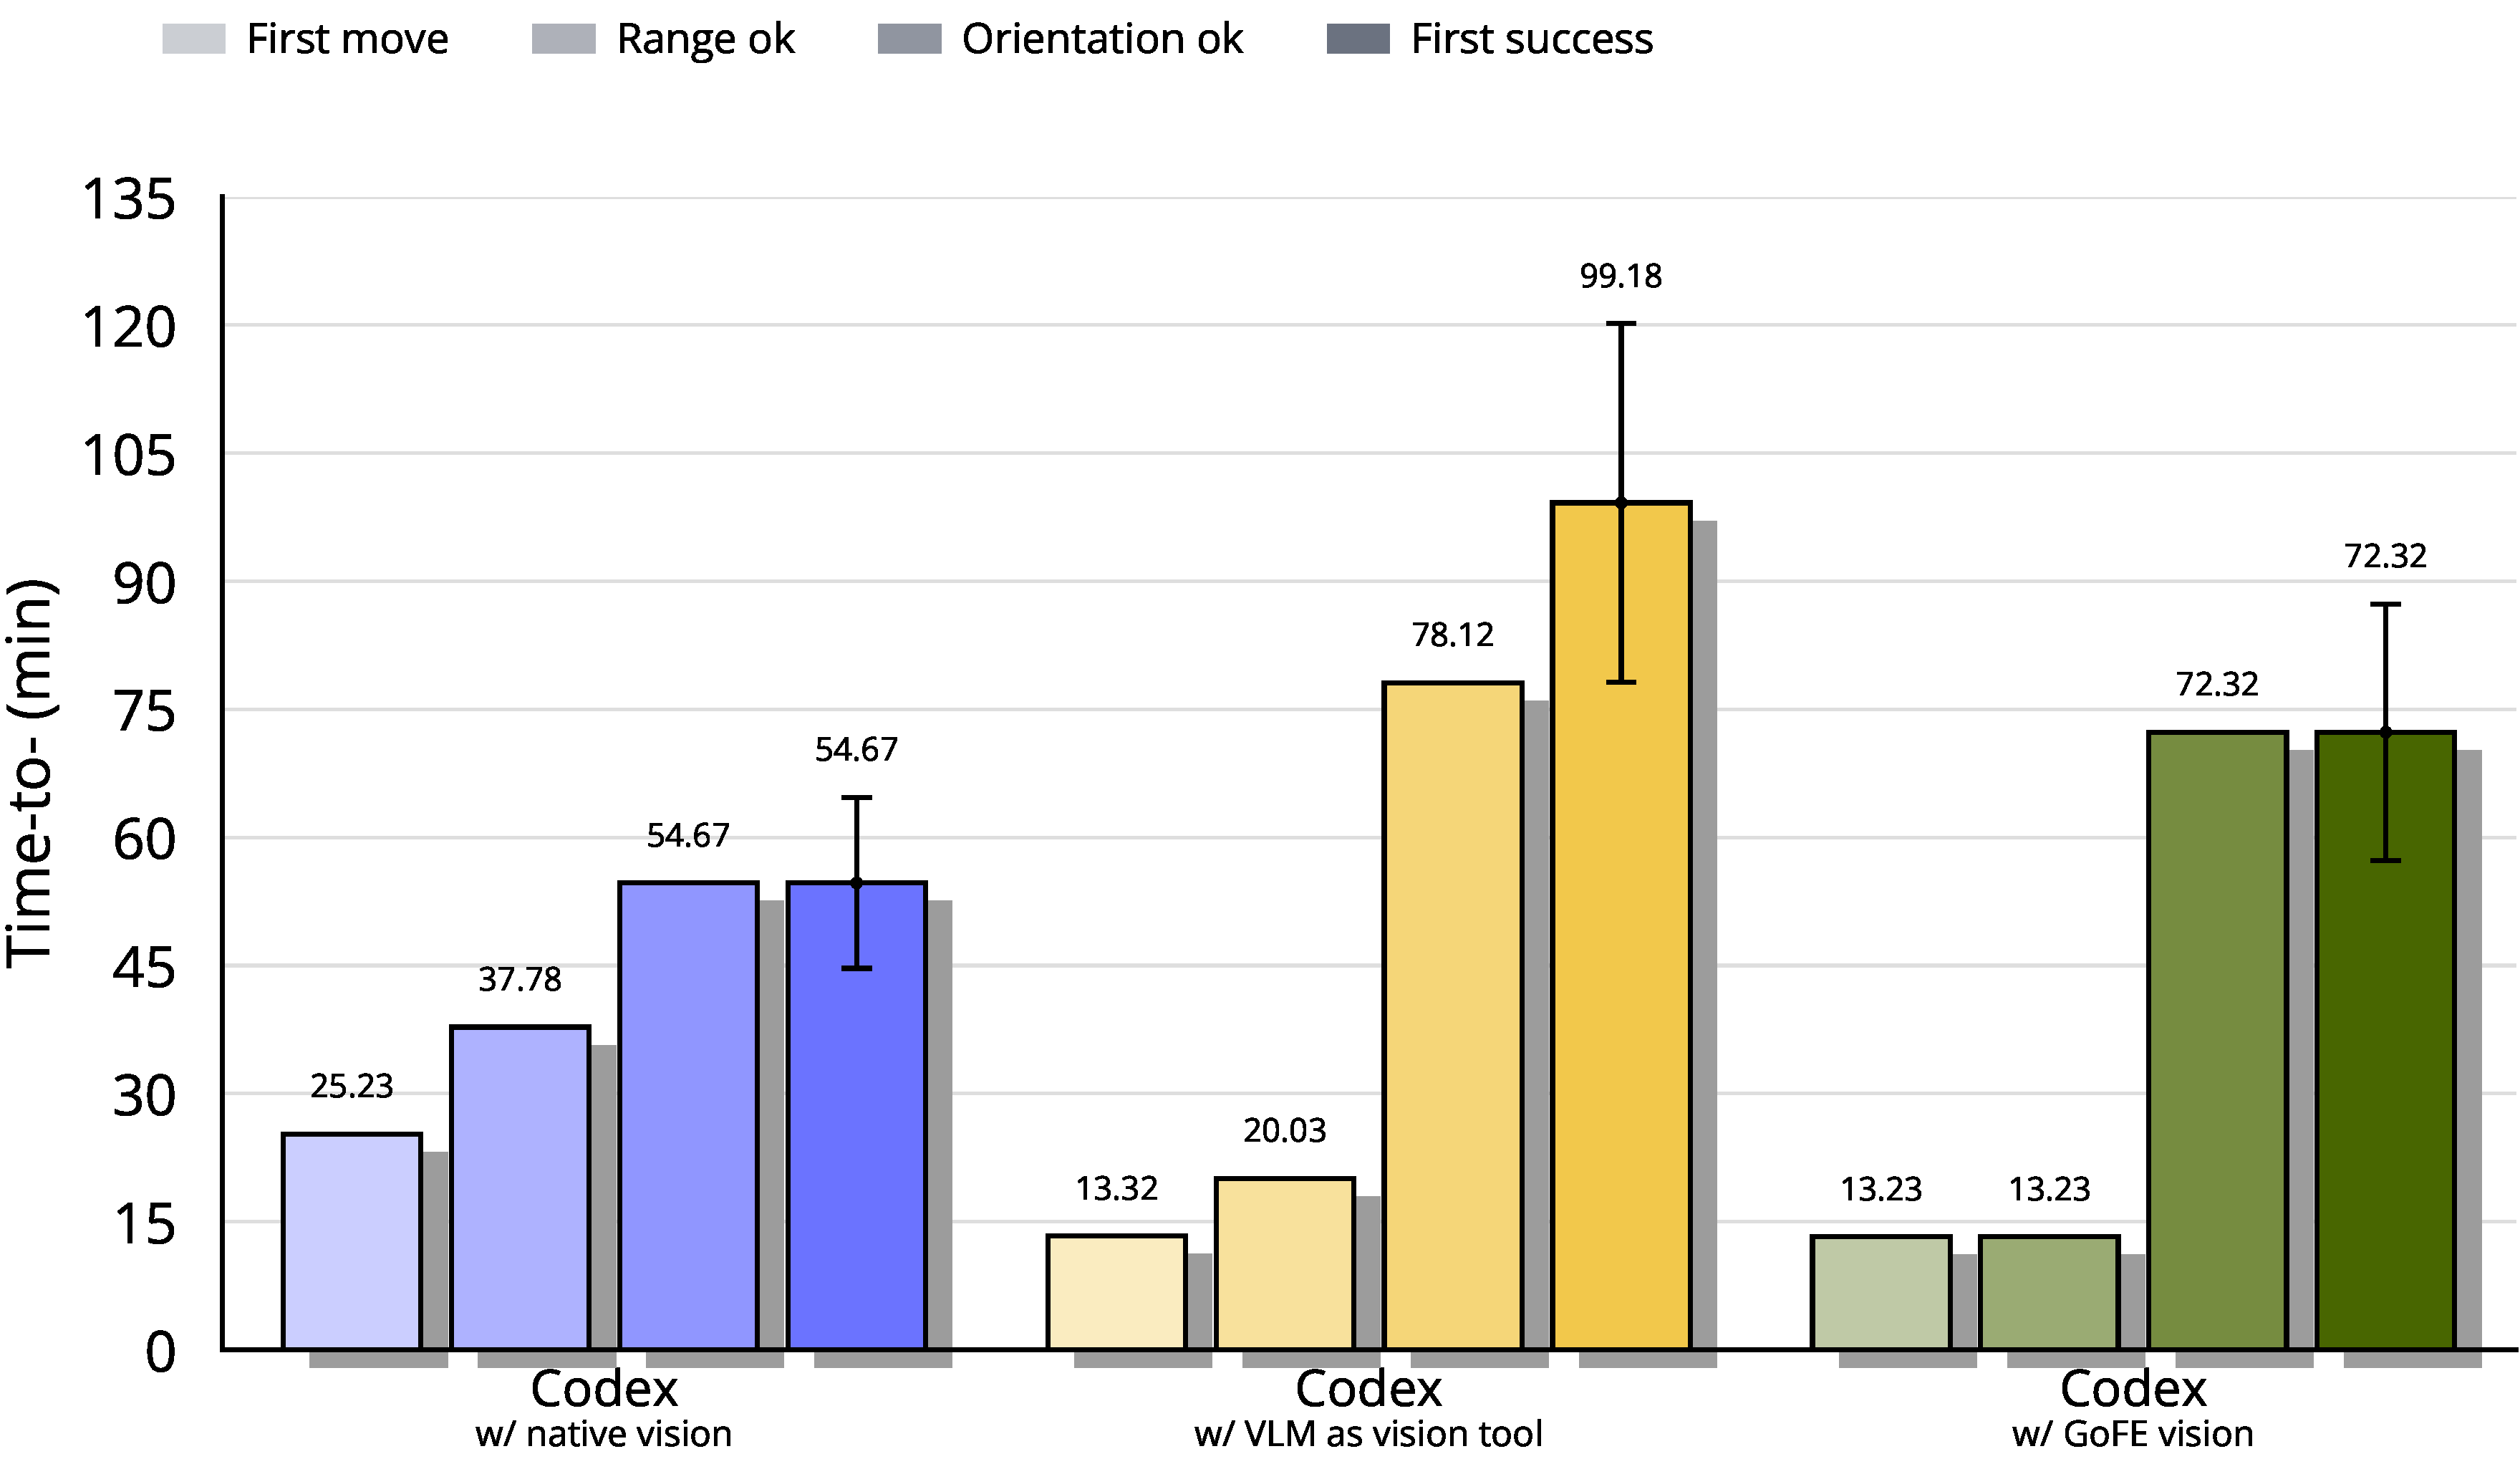
\includegraphics[width=1.0\linewidth]{corl_2026_template_submission//figures/pusht_stage_progress.pdf}
    \caption{Stage-wise progress on the simplified real-world Push-T task under different visual-grounding conditions.}
    \label{fig:pusht_stage_progress}
\end{figure}




Since Push-T requires the agent to localize the object, infer contact geometry, and diagnose failures from evaluation rollouts, we ablate the effect of native vision capability in the coding agent. The Codex harness supports native visual understanding, meaning that the coding agent can directly inspect images. However, many open-source agent harnesses expose only text input. This experiment measures how visual access affects auto-search hill-climbing on the simplified Push-T task. In addition to the original Codex configuration, we evaluated two baselines:

\begin{enumerate}[leftmargin=1.5em]
\item \textbf{Codex without native vision;} We mask image tokens from the coding agent but provide a separate image-understanding module as a callable function. The module reads images, produces descriptions, and answers visual questions; the system prompt is modified to allow the coding agent to call this function when visual information is needed.
\item \textbf{Codex without visual capability.} We remove both native image streaming and visual function calling. In this setting, Codex can only analyze text-based information or write code to extract information from images.
\end{enumerate}

Codex with native vision reaches success first. Surprisingly, the no-vision baseline succeeds before the function-call vision baseline. This suggests that even without direct visual access, the coding agent can infer useful task state from other logging signals, while repeated image function calls introduce additional overhead during task solving.

\begin{figure}
    \centering
    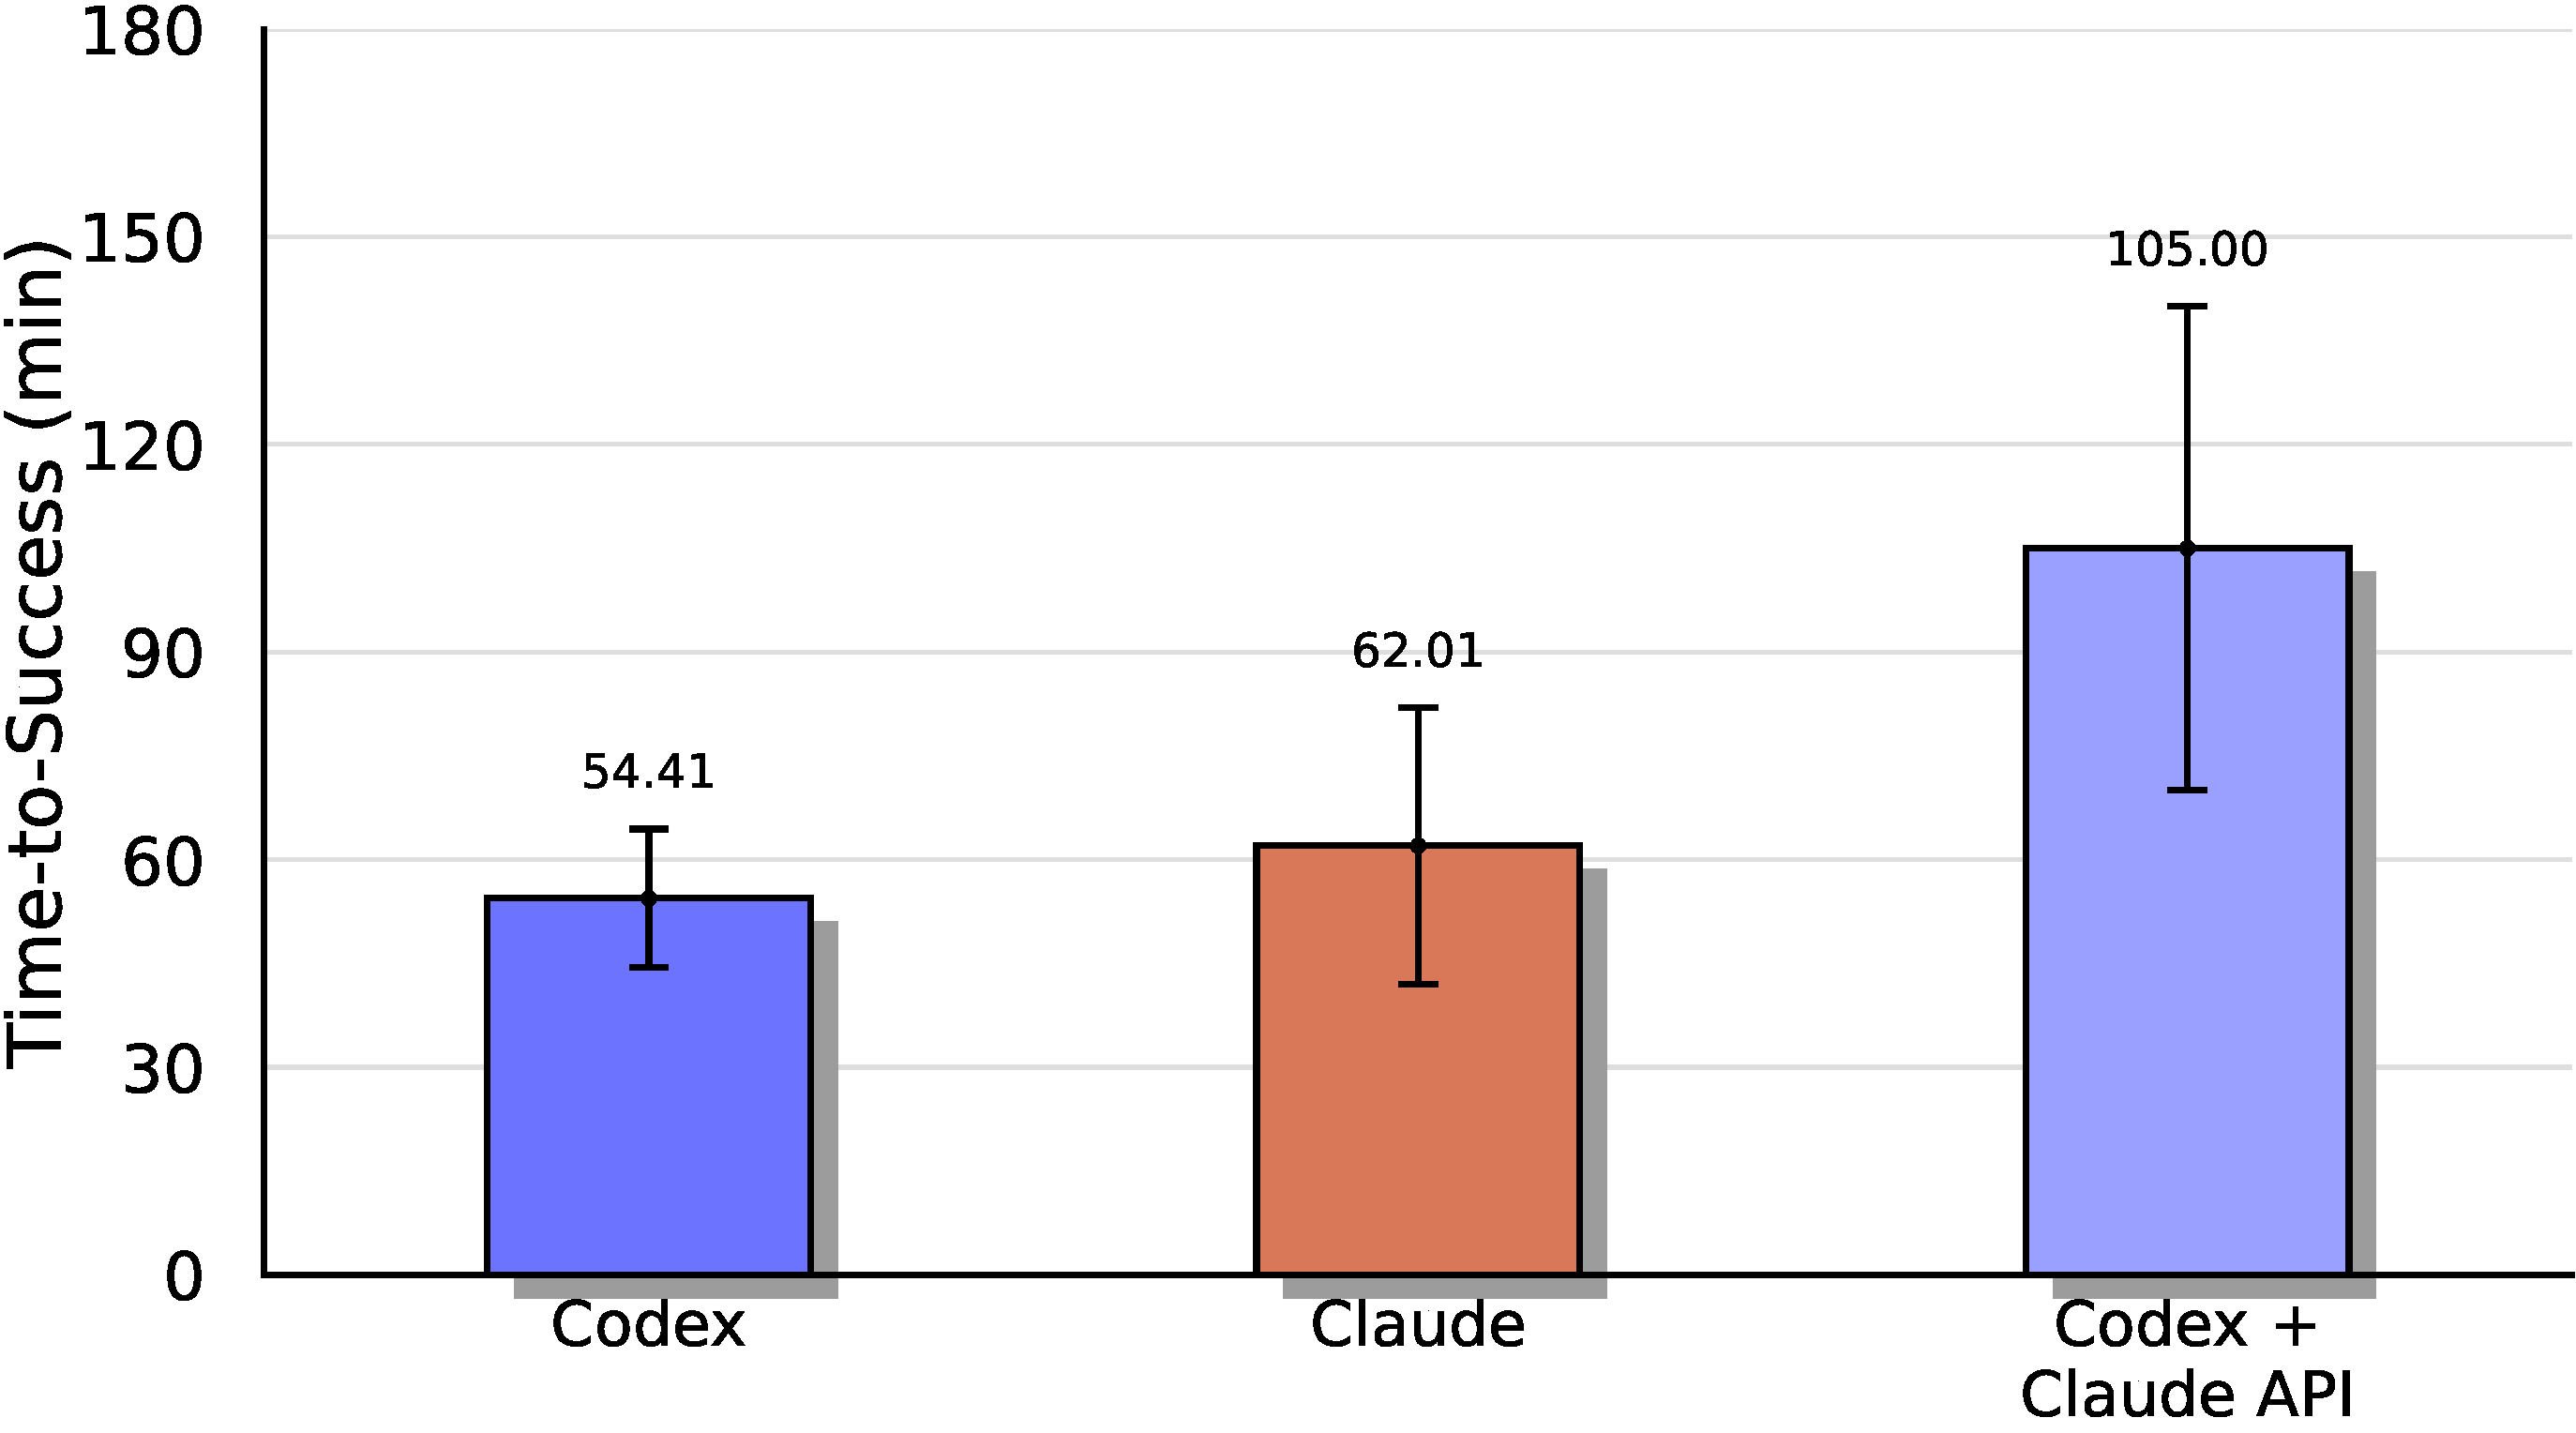
\includegraphics[width=0.5\linewidth]{corl_2026_template_submission//figures/pusht_time_to_success.pdf}
    \caption{Time-to-success comparison across model and agent-harness configurations on the simplified real-world Push-T task. Each configuration is evaluated by the wall-clock time required to reach the predefined success criterion, capturing both model reasoning capability and the practical overhead introduced by the coding interface, tool access, execution loop, and log-inspection workflow.}
    \label{fig:pusht_time_to_success}
\end{figure}

\subsection{Model and Harness Comparison}

We study how the choice of model and agent harness affects end-to-end autoresearch performance. We compare Codex with GPT-5.5, Claude with Opus 4.7, and Codex with Opus 4.7. Codex solves the task fastest, while the Codex harness using the Opus API is the least efficient among the tested configurations.









%----------------------------------------
\section{Simulation Benchmark Result}
\subsection{RoboCasa Simulation Interface and API Surface}
\label{subsec:robocasa-api-summary}

The RoboCasa365 benchmark provides the simulation-side evaluation setting for generated vision-language control scripts. We build middle-level vision and planning stacks on top of the RoboCasa simulation, and encapsulate modular and end-to-end tools as APIs. This interface is injected into generated vision scripts as a single Python namespace. For canonical evaluation scripts, APIs that leak privileged state or enable repeated retries are removed from the runtime namespace. In particular, the environment disables APIs such as \api{get_task_info}, \api{reset_env}, \api{reset_to_initial}, task-specific CLI helpers, and
oracle-target queries. The oracle target API is only exposed outside the canonical script
runtime. \Cref{tab:robocasa-api} summarizes the surface and marks, for each call, whether it is
available in the canonical script runtime (\checkmark) or gated to CLI/oracle modes
(\textsf{C}/\textsf{O}).

{\footnotesize
\setlength{\tabcolsep}{4pt}
\renewcommand{\arraystretch}{1.15}
\begin{longtable}{@{}l p{7.2cm} c@{}}
\caption{RoboCasa environment API surface used in our evaluation. \emph{Avail.}\
indicates availability in the canonical script runtime: \checkmark{} available;
\textsf{C} exposed only in non-canonical CLI mode; \textsf{O} exposed only when the Oracle interface is explicitly enabled.}
\label{tab:robocasa-api}\\
\toprule
\textbf{API} & \textbf{Description} & \textbf{Avail.}\\
\midrule
\endfirsthead
\toprule
\textbf{API} & \textbf{Description} & \textbf{Avail.}\\
\midrule
\endhead
\bottomrule
\endlastfoot

\multicolumn{3}{@{}l}{\textit{State and gripper}}\\
\addlinespace[2pt]
\api{get_robot_state}   & Joint positions, EEF pose, gripper measurement, and base/arm state & \checkmark\\
\api{get_gripper_info}  & Gripper command, measured state, contact bodies, and actuator force & \checkmark\\
\api{set_gripper}       & Set normalized gripper command ($1$ open, $0$ closed) & \checkmark\\
\api{open_gripper}      & Open the gripper & \checkmark\\
\api{close_gripper}     & Close the gripper & \checkmark\\
\addlinespace[3pt]
\multicolumn{3}{@{}l}{\textit{Motion}}\\
\addlinespace[2pt]
\api{move_with_curobo}            & cuRobo plan, OSC waypoint tracking, scene collision & \checkmark\\
\api{move_with_pyroki}            & Pyroki IK with SE(3) interpolation, no scene collision & \checkmark\\
\api{move_with_curobo_joint_exec} & cuRobo plan executed in joint-position mode & \checkmark\\
\api{move_with_pyroki_joint_exec} & Pyroki plan executed in joint-position mode & \checkmark\\
\api{freespace_move}              & Backward-compatible wrapper over configured backend & \checkmark\\
\api{move_eef}                    & Move to a direct end-effector target & \checkmark\\
\api{select_best_grasp}           & Planner-check grasp candidates and select a feasible one & \checkmark\\
\api{go_home}                     & Return to the home configuration & \checkmark\\
\api{nudge}                       & Small local end-effector displacement & \checkmark\\
\api{nudge_brutal}                & Small local move with collision avoidance off & \checkmark\\
\api{rotate_gripper_in_place}     & In-place wrist rotation & \checkmark\\
\addlinespace[3pt]

\multicolumn{3}{@{}l}{\textit{Camera and visualization}}\\
\addlinespace[2pt]
\api{get_camera_image_480_640}      & RGB image at $480\times640$ & \checkmark\\
\api{get_camera_depth_480_640}      & Aligned depth map at $480\times640$ & \checkmark\\
\api{get_camera_intrinsics_480_640} & Intrinsics matched to $480\times640$ & \checkmark\\
\api{get_camera_image}              & Legacy RGB image alias at the environment-native resolution & \checkmark\\
\api{get_camera_depth}              & Legacy depth alias at the environment-native resolution & \checkmark\\
\api{get_camera_intrinsics}         & Legacy intrinsics alias at the environment-native resolution & \checkmark\\
\api{get_camera_extrinsics}         & Camera extrinsics & \checkmark\\
\api{set_debug_markers}             & Place visualization markers & \checkmark\\
\addlinespace[3pt]

\multicolumn{3}{@{}l}{\textit{Perception}}\\
\addlinespace[2pt]
\api{detect_object}               & Text-conditioned object detection & \checkmark\\
\api{segment_object}              & Single-instance segmentation & \checkmark\\
\api{segment_object_all}          & Multi-instance segmentation & \checkmark\\
\api{detect_objects_oneshot}      & One-shot object detection & \checkmark\\
\api{sample_grasp_pose_anygrasp}  & AnyGrasp grasp-pose sampling & \checkmark\\
\api{vlm_query}                   & Vision-language model query & \checkmark\\
\addlinespace[3pt]

\multicolumn{3}{@{}l}{\textit{Planner and collision}}\\
\addlinespace[2pt]
\api{update_planner_world}    & Set the cuRobo collision geometry & \checkmark\\
\api{refresh_planner_world}   & Refresh collision geometry from the scene & \checkmark\\
\api{disable_collision_avoid} & Disable collision avoidance & \checkmark\\
\addlinespace[3pt]

\multicolumn{3}{@{}l}{\textit{Task, policy, and navigation}}\\
\addlinespace[2pt]
\api{get_task_description}    & Natural-language task instruction & \checkmark\\
\api{use_policy_output}       & Query an external policy's output & \checkmark\\
\api{get_base_state}          & Mobile-base state & \checkmark\\
\api{execute_base_trajectory} & Execute a planned base trajectory & \checkmark\\
\api{create_goat_agent}       & Instantiate a GOAT navigation agent & \checkmark\\
\api{set_goat_goal}           & Set the GOAT navigation goal & \checkmark\\
\api{goat_navigate}           & Run GOAT navigation & \checkmark\\
\api{get_goat_state}          & Return GOAT state and configuration & \checkmark\\
\api{reset_goat}              & Reset GOAT state & \checkmark\\
\addlinespace[3pt]

\multicolumn{3}{@{}l}{\textit{Utilities}}\\
\addlinespace[2pt]
\api{display_rpy_to_quat} & Convert display RPY angles to an \api{xyzw} quaternion & \checkmark\\
\api{np}, \api{numpy}      & NumPy convenience exports for generated scripts & \checkmark\\
\addlinespace[3pt]

\multicolumn{3}{@{}l}{\textit{Gated / removed in the canonical script runtime}}\\
\addlinespace[2pt]
\api{get_task_info}      & Structured task information & \textsf{C}\\
\api{reset_env}          & Reset the environment & \textsf{C}\\
\api{reset_to_initial}   & Reset to the initial state & \textsf{C}\\
\api{get_oracle_targets} & Ground-truth target pose / oracle query & \textsf{O}\\
\end{longtable}
}

\paragraph{Camera and visualization.}
The camera APIs provide RGB-D observations, camera intrinsics, and extrinsics. We use resolution-specific calls to keep RGB, depth, and intrinsics mutually aligned, while retaining unsuffixed aliases for backward compatibility. Debug markers are used only for visualizing intermediate targets during development.

\paragraph{Motion.}
The motion APIs provide both cuRobo- and Pyroki-based execution. cuRobo uses scene collision geometry and is the default choice for free-space manipulation, whereas Pyroki provides lightweight SE(3) interpolation with inverse kinematics but no scene-level collision model. The standard mode
tracks end-effector waypoints with OSC, while joint-execution variants are used when faithfully following the planned joint path is important, such as near joint limits or tight obstacles.

\paragraph{Perception.}
The perception APIs provide text-conditioned detection, segmentation, one-shot detection,
grasp-pose sampling, and vision-language queries. These calls allow generated scripts to ground
language instructions in visual observations without accessing the simulator ground truth.

\paragraph{Planner and collision.}
The planner APIs maintain the cuRobo collision geometry from the simulated scene. Collision
avoidance is enabled by default for ordinary free-space motion, and collision disabling is reserved
for short, intentional contact-rich actions or known collision-model artifacts.

\subsection{RoboCasa Evaluation Protocol}
\label{subsec:robocasa-eval-protocol}

We evaluate each RoboCasa task in simulation using the same environment wrapper
and script runtime described above. Each script generated by the coding agent is executed
once per episode through the canonical evaluation harness. The harness creates
the RoboCasa environment, injects the restricted Python tool namespace into the
script, runs the script to completion, records videos and logs, and then queries
the environment's native success function for the final score. We report binary
task success as defined by RoboCasa's native success predication: an episode is
counted as successful when this predicate returns true at the end of execution.

\paragraph{Fixed seeds and layouts.}
For each reported 40-episode evaluation, we use a fixed list of seed triplets.
Each triplet contains a RoboCasa random seed, a layout identifier, and a style
identifier: \texttt{\detokenize{(seed, layout_id, style_id)}}.
The 40 triplets are generated once using a deterministic seed-list generator
with generator seed 42, and then saved as a static evaluation file. For all
reported evaluations, including smaller diagnostic subsets, we use rows from
this saved file rather than regenerating a new list, so that subsets are
prefixes or explicit selections from the same canonical 40-episode benchmark.
The same triplet list is used for all methods compared on a task.


\paragraph{Fair comparison with GR00T.}
When comparing generated vision scripts with GR00T, we use the same task name,
same seed triplets, same initial simulator states, same camera configuration,
and same RoboCasa success predicate. GR00T and the vision scripts are therefore
scored on matched episodes rather than on separately sampled scenes. The task
language prompt is the same RoboCasa instruction, and neither method receives
oracle target poses or simulator object states during execution. The methods
differ in their execution pathway: GR00T acts through its learned policy
rollout, while the generated scripts compose the public perception, planning,
and manipulation APIs listed in \Cref{tab:robocasa-api}. We report success over the same fixed evaluation set so that differences reflect the policy or script behavior rather than different scene sampling or privileged information.

\paragraph{Discovered policy demonstration.}
In addition to the matched-seed success rates reported in the main paper, the
project website at \website includes qualitative
demonstrations of the coding-agent-discovered policy. In particular, the videos
show the agent-discovered strategy of combining detection and motion planning to
move the gripper to a hover pose above the target object before grasping, which
is the RoboCasa strategy transferred to the real-world scissors and zip tie
task in the main paper.

\begin{figure}
    \centering
    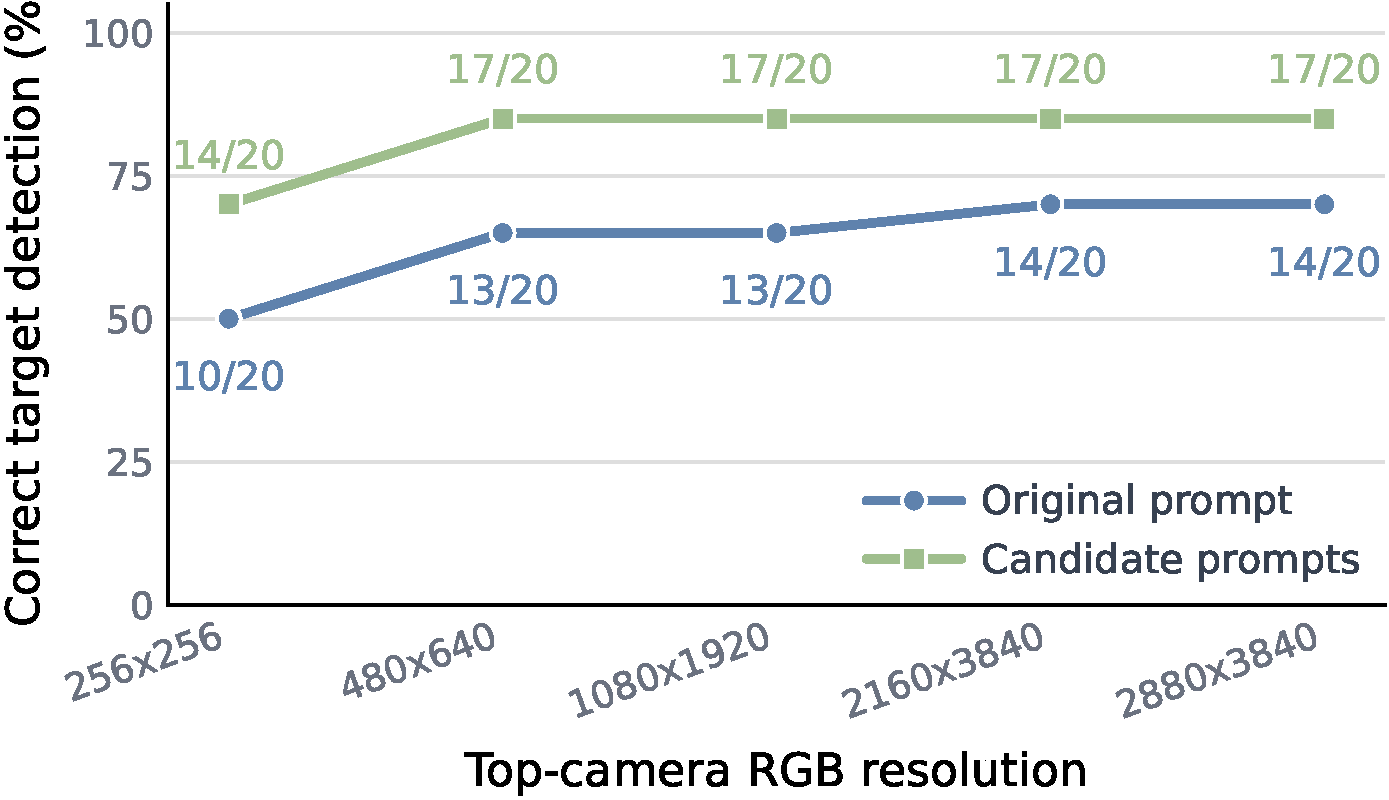
\includegraphics[width=0.8\linewidth]{corl_2026_template_submission//figures/sam3_counter_to_cabinet_correctness_target_sr_by_resolution_line.pdf}
    \caption{SAM3 target-object detection accuracy on RoboCasa counter-to-cabinet scenes as a function of top-camera RGB resolution. Each point evaluates 20 target-object queries. The original task prompt improves from 10/20 correct detections at $256\times256$ to 14/20 at higher resolutions, while candidate prompts generated by the coding agent improve from 14/20 to 17/20 and then plateau.}
    \label{fig:robocasa_sam3_resolution}
\end{figure}

\begin{figure}
    \centering
    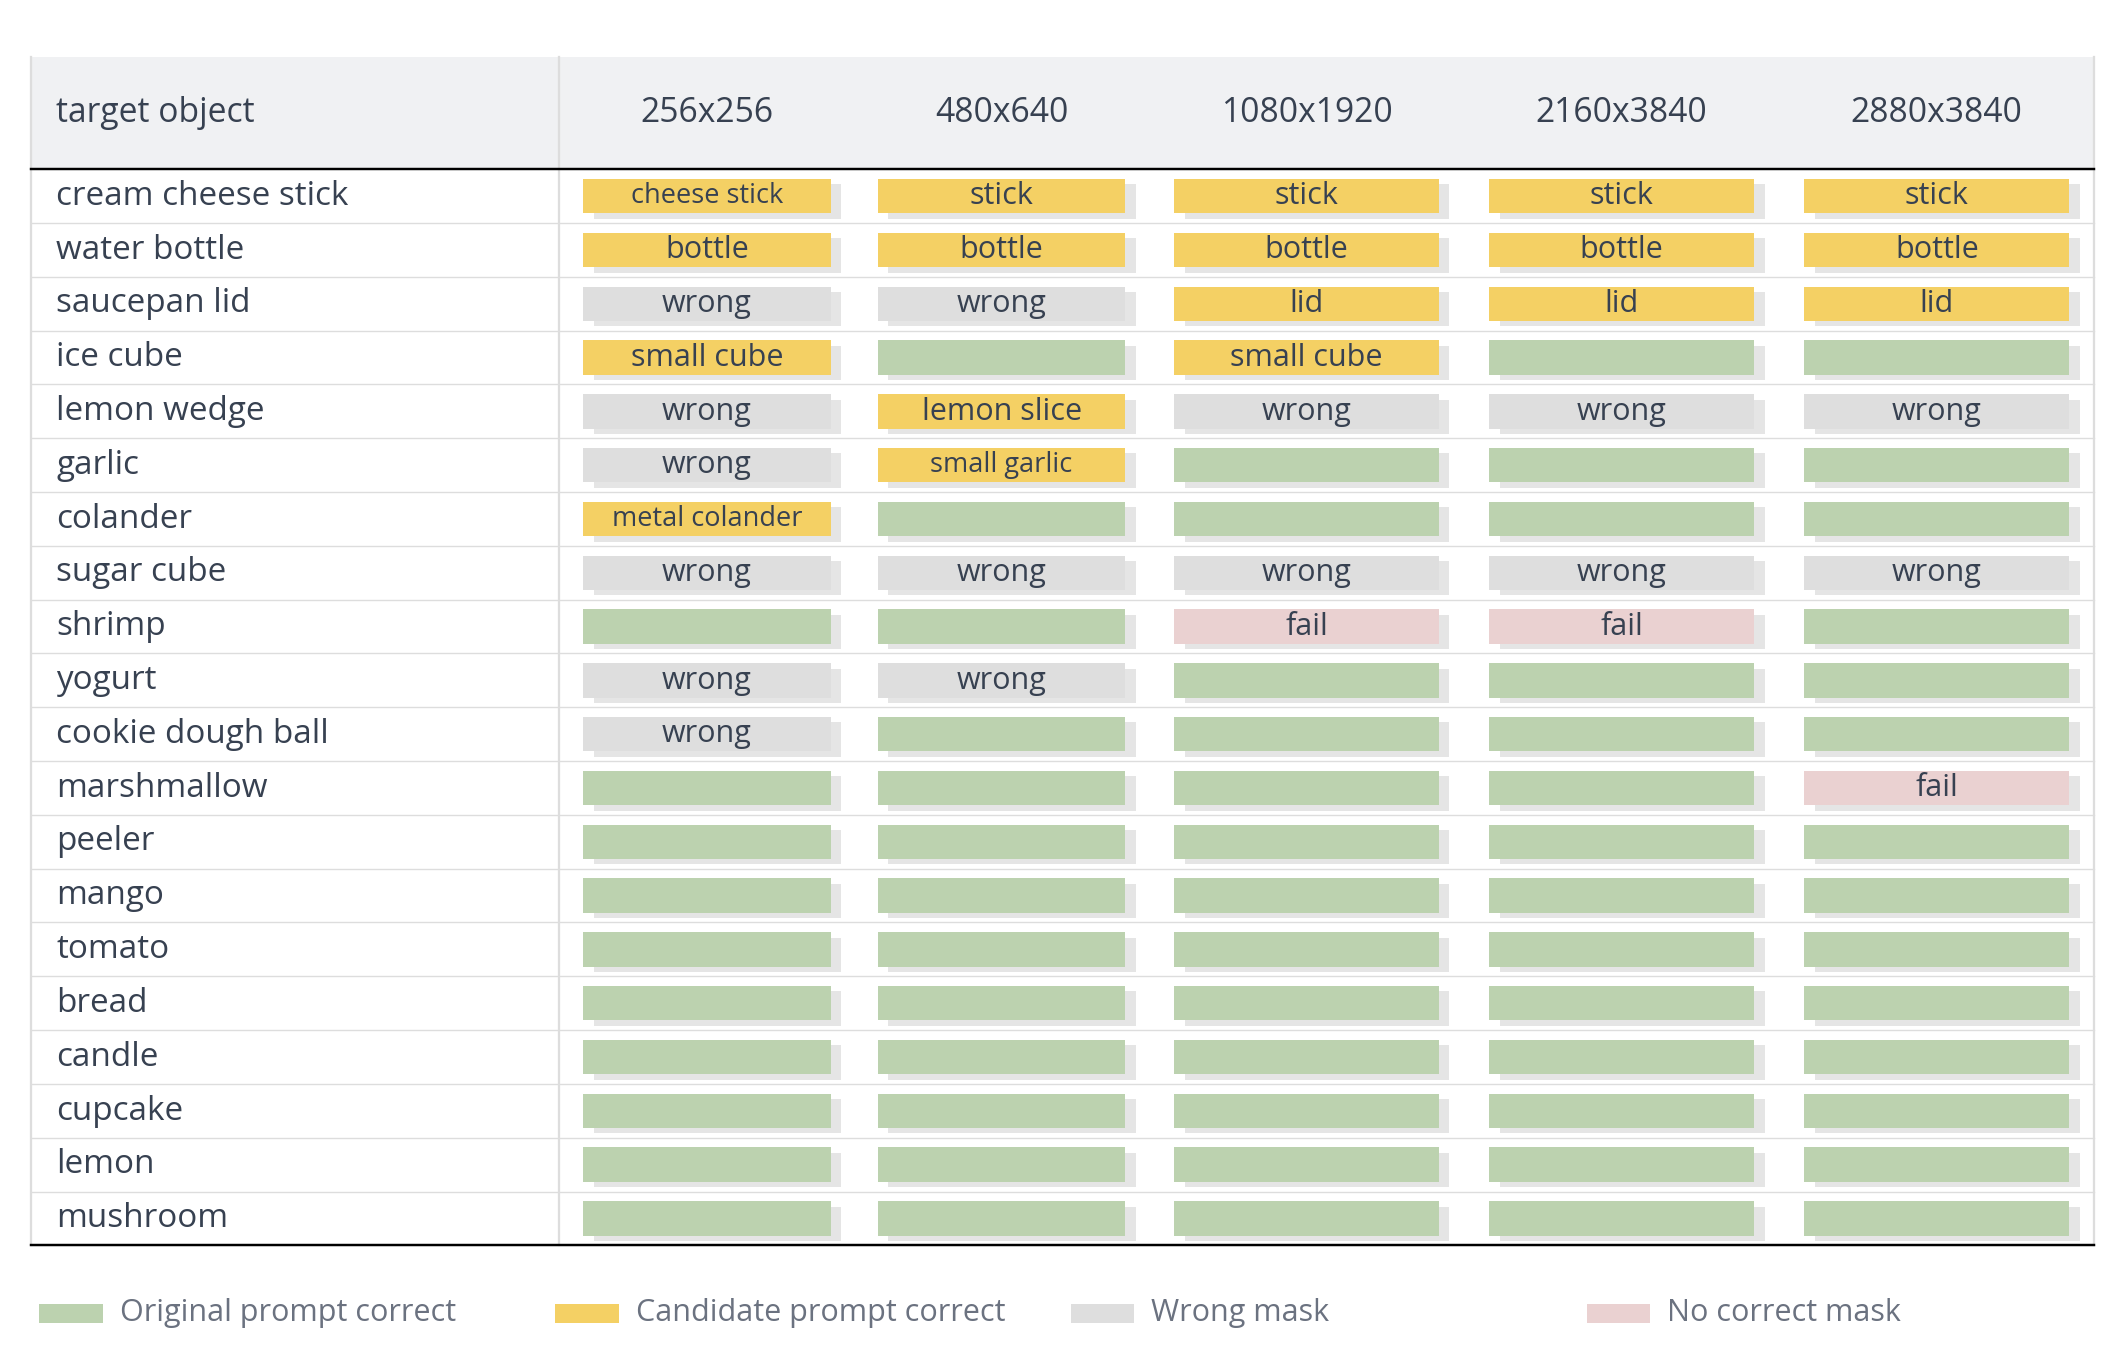
\includegraphics[width=0.9\linewidth]{corl_2026_template_submission//figures/sam3_counter_to_cabinet_correctness_prompt_table_by_resolution.png}
    \caption{Per-object SAM3 detection outcomes across top-camera resolutions and prompt variants for the RoboCasa counter-to-cabinet diagnostic set. Green cells indicate that the original target prompt produced a correct mask, yellow cells indicate that a candidate prompt produced a correct mask, gray cells indicate an incorrect mask, and red cells indicate that no correct mask was returned.}
    \label{fig:robocasa_sam3_prompt_table}
\end{figure}

\begin{figure}
    \centering
    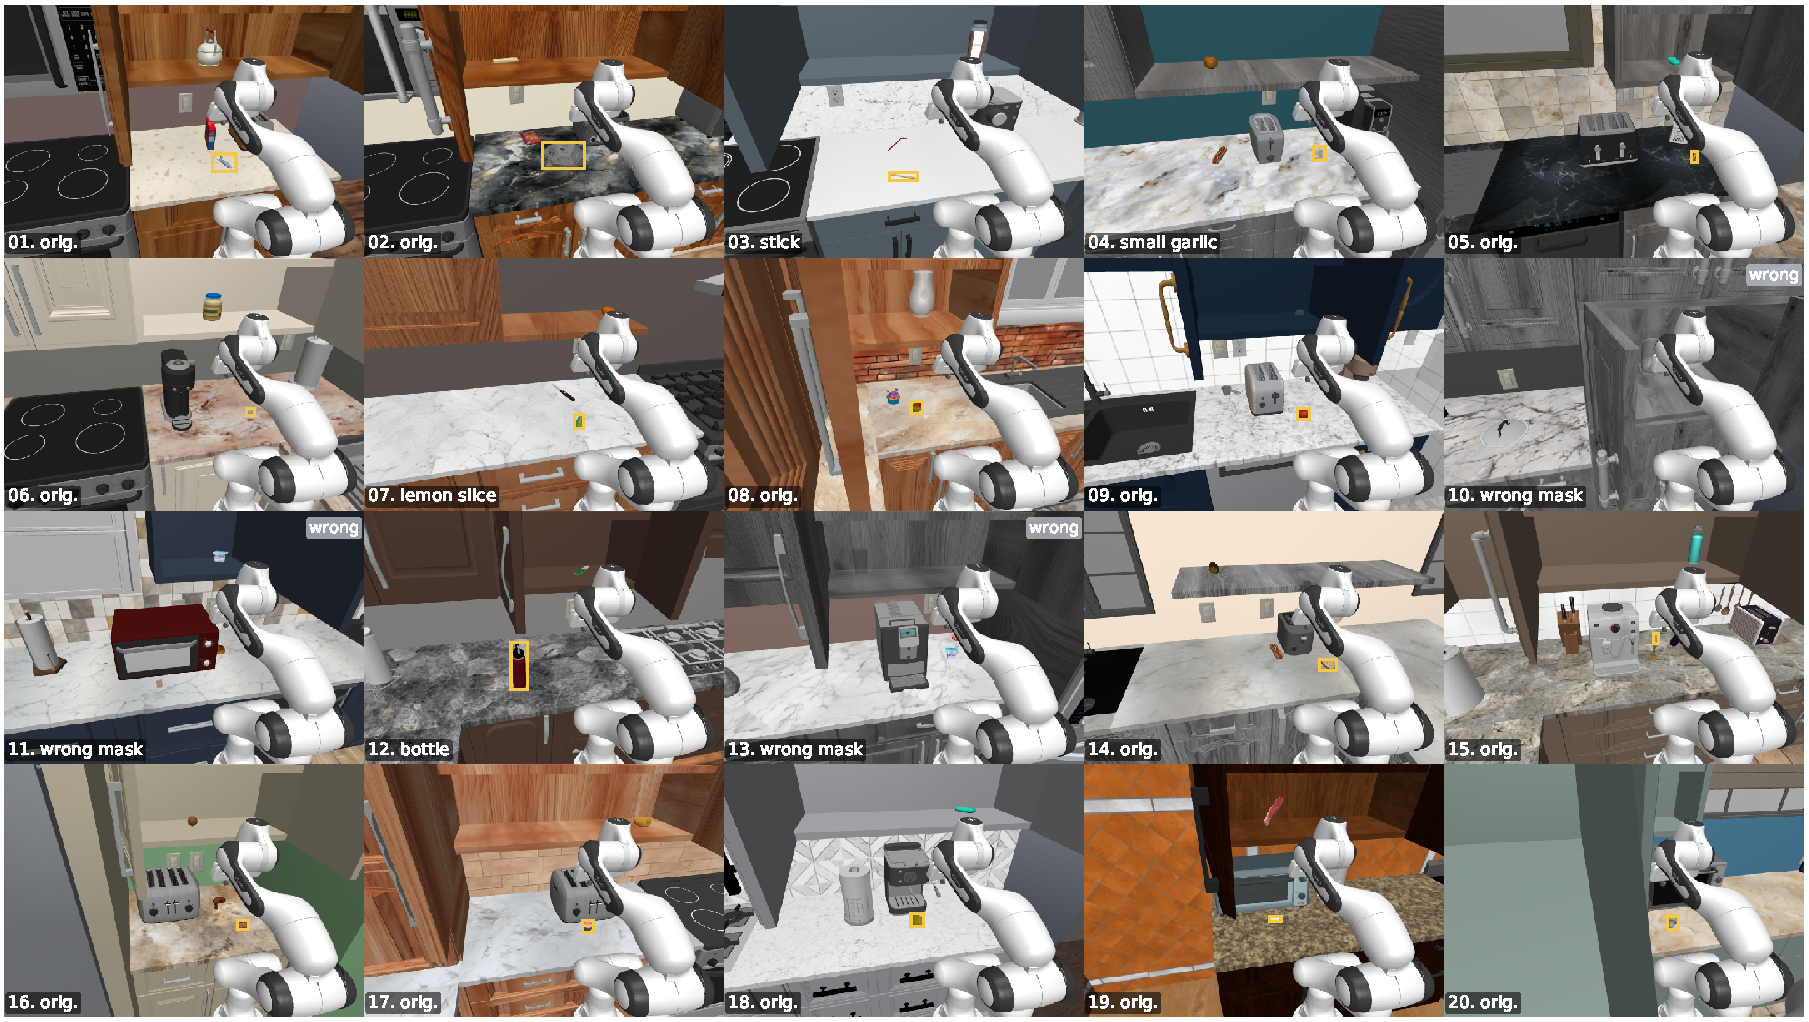
\includegraphics[width=1\linewidth]{corl_2026_template_submission//figures/sam3_counter_to_cabinet_correctness_prompt_bbox_grid_480x640.pdf}
    \caption{Qualitative SAM3 mask outputs for 20 RoboCasa counter-to-cabinet target objects at $480\times640$ resolution. Yellow boxes show selected target masks; labels indicate whether the original prompt, a candidate prompt, or a wrong mask was used.}
    \label{fig:robocasa_sam3_bbox_grid}
\end{figure}

\paragraph{Result Analysis}
We identified a perception bottleneck in which SAM3 can return an incorrect mask or no usable mask for small or ambiguous RoboCasa objects. \Cref{fig:robocasa_sam3_resolution,fig:robocasa_sam3_bbox_grid} isolate this effect by varying image resolution and prompt wording on the same counter-to-cabinet diagnostic set. Increasing the top-camera resolution from $256\times256$ to $480\times640$ improves detection, but resolution alone does not solve all failures. Allowing the coding agent to rewrite object prompts further improves target detection and recovers several cases where the original task wording produces a distractor mask. This analysis shows that generated RoboCasa scripts are limited not only by planning and control, but also by the reliability of the perception API exposed to the agent; prompt search and resolution selection are therefore useful parts of the agent's simulation-side tool use.

